\documentclass[11pt]{article}
\usepackage[UTF8]{ctex}
\usepackage[margin=1in]{geometry}
\usepackage{amsfonts,amsmath,amssymb}
\usepackage[none]{hyphenat}
\usepackage{fancyhdr}
\usepackage{graphicx}
\usepackage{float}
\usepackage{booktabs}
\usepackage{array}
\usepackage{emptypage}
\usepackage{subfigure}
\usepackage{longtable}
\usepackage{listings}
\usepackage{xcolor}
\usepackage{multirow}

\lstset{
    numbers=left, 
    numberstyle= \tiny, 
    keywordstyle= \color{ blue!70},
    commentstyle= \color{red!50!green!50!blue!50}, 
    frame=shadowbox,
    rulesepcolor= \color{ red!20!green!20!blue!20} ,
    escapeinside=``, 
    xleftmargin=2em,xrightmargin=2em, aboveskip=1em,
    framexleftmargin=2em
}

\lstset{language=MATLAB}
\lstset{breaklines}
\lstset{extendedchars=false}

\pagestyle{fancy}
\fancyhead{}
\fancyfoot{}
\fancyhead[LE]{\slshape \MakeUppercase{\leftmark}}
\fancyhead[OR]{\slshape{\rightmark}}
\fancyfoot[C]{\thepage}
\renewcommand{\headrulewidth}{0.5pt}

\setlength{\parindent}{4em}
\setlength{\parskip}{1em}
\renewcommand{\baselinestretch}{1.5}
\renewcommand{\abstractname}{\large Abstract\\}
\renewcommand\refname{Reference}
%\setcounter{secnumdepth}{1}
%\setcounter{tocdepth}{1}
\begin{document}
\cleardoublepage
\begin{titlepage}
\begin{center}
\vspace*{1cm}
\Large{\textbf{MATLAB}}\\
\Large{\textbf{Assignment Series}}\\
\vfill
\line(1,0){400}\\[1mm]
\huge{\textbf{The Project}}\\[3mm]
\Large{\textbf{-The Research on Students' Admission in India-}}\\[1mm]
\line(1,0){400}
\vfill
By Kinsgley Cheng\\
Student ID: 202228000243001\\
Academy of Mathematics and System Science\\
\today \\
\end{center}
\end{titlepage}
\begin{abstract}
	本文主要通过建立多元线性回归模型研究影响印度本科学生升学录取机率的因素,研究的因素范围包括GRE成绩、TOFEL 成绩、大学评分、个人陈述、推荐信、本科 GPA 和科研经历这7个因素。
	
	首先,我们对数据进行预处理,画出各变量的频数直方图、箱型图、计算各变量的基本统计量,包括最大值、最小值、中位数和众数、画出各变量之间的相关热力图。从而能够对所处理数据的分布状况、相关性和异常值的情况有一个初步的了解。
	
	接下来,我们对回归方程进行全模型回归,了解数据的整体线性性质,以测试线性回归模型的可行性,发现方程整体显著性高,只存在少量变量不显著。这说明该问题大致可以采用线性模型进行解释。为了处理不显著的变量,我们依次采用逐步回归、LASSO 回归、Elastic Net 等方法分别进行变量选择,期望通过统计性质剔除不相关因素,以提高模型整体的拟合度与可解释性。通过比较各种方法的结果,我们发现在这里 LASSO 回归与 Elastci Net 对变量的分离性能并不太好,所以最终采用了逐步回归的结果,即删除变量---个人陈述。
	
	然后,我们对变量选择后的子集重新进行回归,对得到的回归方程进行统计性检验。首先进行异方差诊断。在画出残差散点图后,无法判断其异方差性,接着分别采用 Spearman 检验和 White 检验分别对回归方程的变量和整体进行诊断,发现方程存在严重异方差。对此,我们采用 BOX-COX 变换进行处理,通过极大似然最小 MSE 的方法选取$\lambda$,处理后发现重新检验,发现异方差已消除。
	
	下一步,我们进行自相关检验。我们画出残差时序图,初步判断回归方程可能存在一定自相关性,再通过 DW 检验,进一步确定了模型自相关性的存在。我们再一次观测时序图,发现残差间存在近似线性相关性,故推断其存在一阶自相关,进而采用迭代法进行处理,处理后再次进行检验,发现方程自相关性被消除。
	
	最后,我们对所得的回归方程,进行多重共线性的检验。主要是计算其方差膨胀因子(VIF)和条件数,发现不存在共线性,至此回归方程建立完成。
	
	对于上述得到的回归方程,我们进行初步的回归诊断,分别画出其学生化残差散点图、Cook距离散点图和各个杠杆值相较于平均杠杆值倍数的散点图,基本判断回归方程存在极少的异常值,但可能存在一定的高杠杆值点。
	
	最后通过得到的回归方程,我们对模型进行一定的初步解释。可以发现,对于印度学生而言,大学的录取率和个人推荐信的好坏并没有很大的关系,而和本科GPA与是否具有科研经历具有密切关系。
	
\par\noindent\textbf{Keywords: 多元线性回归、变量选择、BOX-COX变换、升学录取}
\end{abstract}	
\newpage
\thispagestyle{empty} %no header
\begin{center}
	\tableofcontents
\end{center}
\thispagestyle{empty}
\newpage
\setcounter{page}{1}
\section{问题背景}
对于每一个学生而言,大学的选择与录取都对他们今后的人生发展有着至关重要的影响。而大学的录取率受多种因素影响,且其中的关系复发,预测每位学生的录取机率是一个极其复杂的问题。相关部门经过初步调查和对往年录取情况的一定的研究分析后,发现学校的录取与否主要取决于 GRE 成绩、TOFEL 成绩、大学评分、个人陈述、推荐信、本科 GPA 和科研经历这 7 个因素的相关性较高。

现在我们有 500 名印度学生的 7 项指标与他们的录取机率的数据\footnote{data is from Mohan S Acharya, Asfia Armaan, Aneeta S Antony : A Comparison of Regression Models for Prediction of Graduate Admissions, IEEE International Conference on Computational Intelligence in Data Science 2019},我们希望借此建立线性回归模型,能够帮助将来的学生更加清晰准确地来预测与评估自己的录取机率,以便更有效及时的获取大学的录取。与此同时,也希望给一些在籍本科生提供准备方向的参考和侧重,能够在将来申请时到更好的结果。
\section{基本假设}
对于所处理的问题与建立的模型,我们有如下几条基本假设:
\begin{itemize}
	\item[1.] 假定数据的来源均真实可靠,录入与统计误差不会对模型产生严重的影响。
	\item[2.] 假定 500 名学生相互独立,各个数据间不存在相关关系。
	\item[3.] 假定各个学校对于每个学生的推荐信和个人陈述的评分尺度一致,不存在主观人为因素,各个学校间的差异可以忽略。同时,数据中的大学评分与录取几率的评估具有一定的权威性,即能够反应真实情况。
\end{itemize}
\section{符号说明}
\begin{longtable}[H]{cccc}
	\hline
	变量符号&变量含义&取值范围&单位\\
	\hline
	n&学生序号&1、2、$\cdots$、500&/\\
	$x_1$&GRE成绩& 0$\sim$340&分\\
	$x_2$&TOEFL成绩&0$\sim$120&分\\
	$x_3$&大学评分&1、2、3、4、5&分\\
	$x_4$&个人陈述评分(SOP)&1、2、3、4、5&分\\
	$x_5$&推荐信评分(LOR)&1、2、3、4、5&分\\
	$x_6$&本科GPA(CGPA)&0$\sim$10&/\\
	$x_7$&科研经历&0、1&/\\
	$y$&录取机率&0$\sim$1&/\\
	\hline
\end{longtable}

\section{模型建立与求解}
\subsection{数据预处理与基本分析}
\subsubsection*{缺失值检验}
首先我们需要对数据进行缺失值检验。通过检验,可以发现原数据集并无缺失值存在。
\subsubsection*{直方图---数据分布形态的分析}
接下来,我们分别做出各变量的频率直方图,以此来了解数据的大致分布情况。
\begin{figure}[H]
	\centering
	\caption{前四个变量的直方图}
	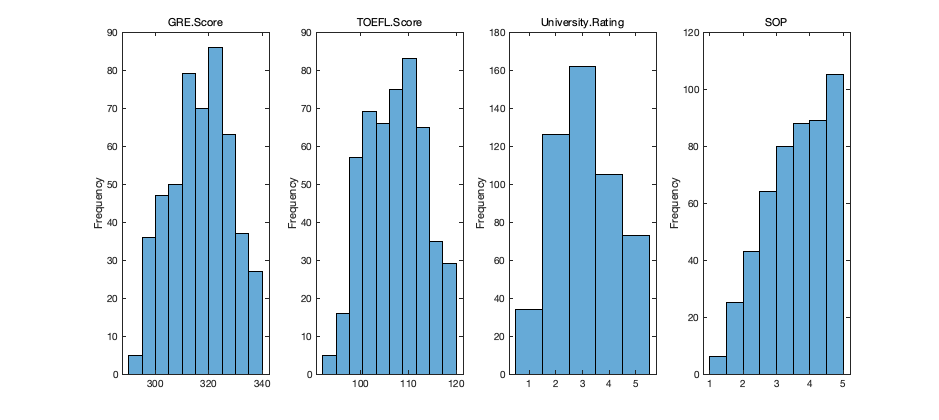
\includegraphics[scale=0.43]{images/histgraph1.png}
\end{figure}
\begin{figure}[H]
	\centering
	\caption{后三个变量的直方图}
	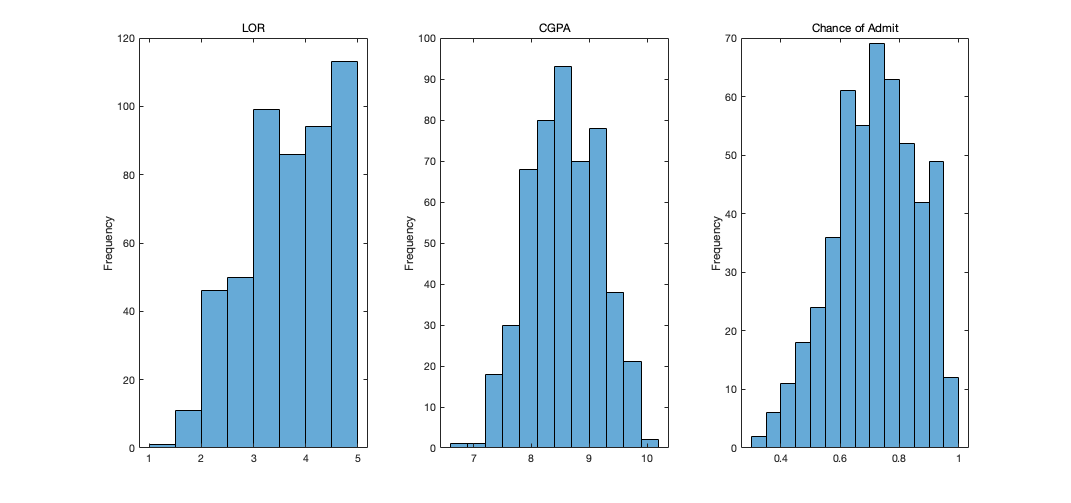
\includegraphics[scale=0.35]{images/histgraph2.png}
\end{figure}
\subsubsection*{基本统计量}
我们可以计算出各变量的基本统计量,结果统计如下:
\begin{table}[H]
	\centering
	\caption{各变量的基本统计量}
	\begin{tabular}{ccccccccc}
		\hline\hline
		变量&$x_1$&$x_2$&$x_3$&$x_4$&$x_5$&$x_6$&$x_7$&y\\
		\hline
		最大值&340.0&120.0&5.0&5.0&5.0&9.9&1.0&0.97\\
		最小值&290.0&92.0&1.0&1.0&1.0&6.8&0.0&0.34\\
		平均值&316.5&107.2&3.1&3.4&3.5&8.6&0.6&0.72\\
		中位数&317&107.0&3.0&3.5&3.5&8.6&81.0&0.72\\
		\hline\hline
	\end{tabular}
\end{table}
\subsubsection*{箱形图---异常值初步判断}
下面我们画出箱型图,对一些异常值进行初步判断
\begin{figure}[H]
	\centering
	\caption{前4个变量的箱形图}
	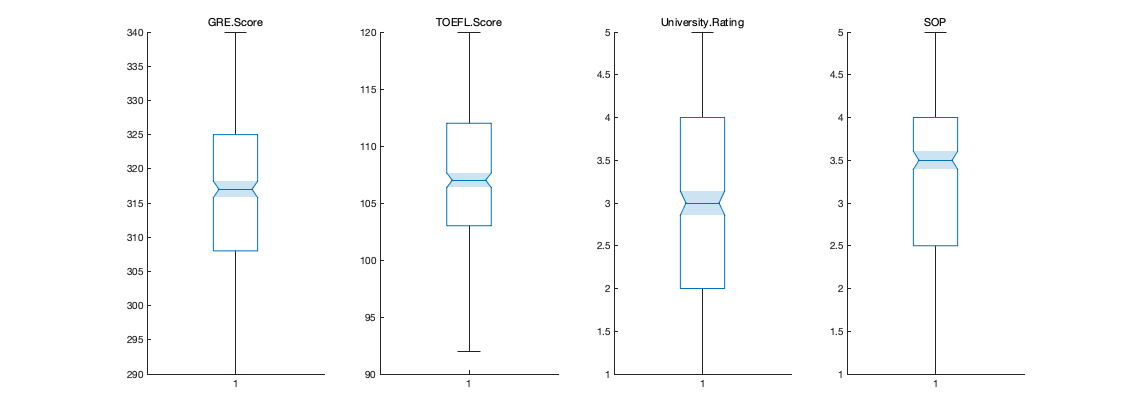
\includegraphics[scale=0.35]{images/boxplot1.png}
\end{figure}
\begin{figure}[H]
	\centering
	\caption{后3个变量的箱形图}
	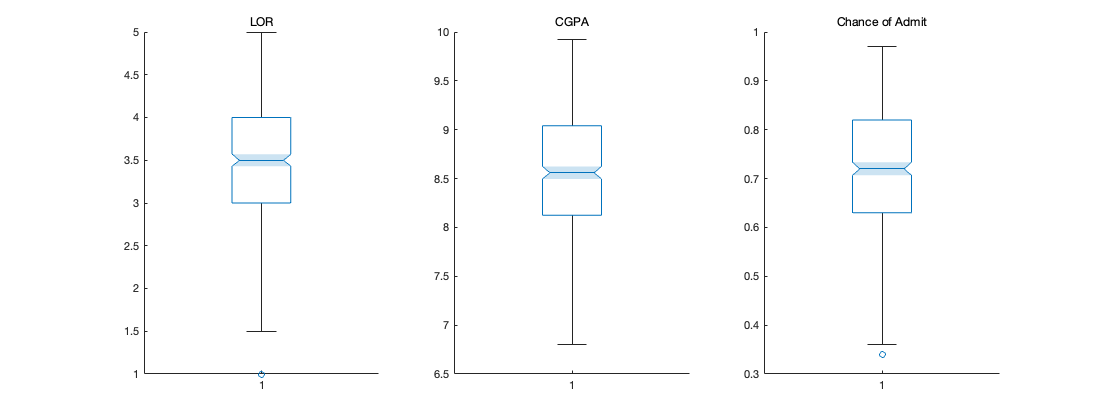
\includegraphics[scale=0.35]{images/boxplot2.png}
\end{figure}

通过箱形图我们可以发现变量LOR和因变量录取几率存在异常值,考虑到异常值数量较少,我们将其删除(93、348、377  行数据)。
\subsubsection*{相关热力图---变量相关性的初步分析}
下面我们画出各变量之间的热力图,对它们之间的线性相关性有一个比较直观地了解。
\begin{figure}[H]
	\centering
	\caption{相关系数热力图}
	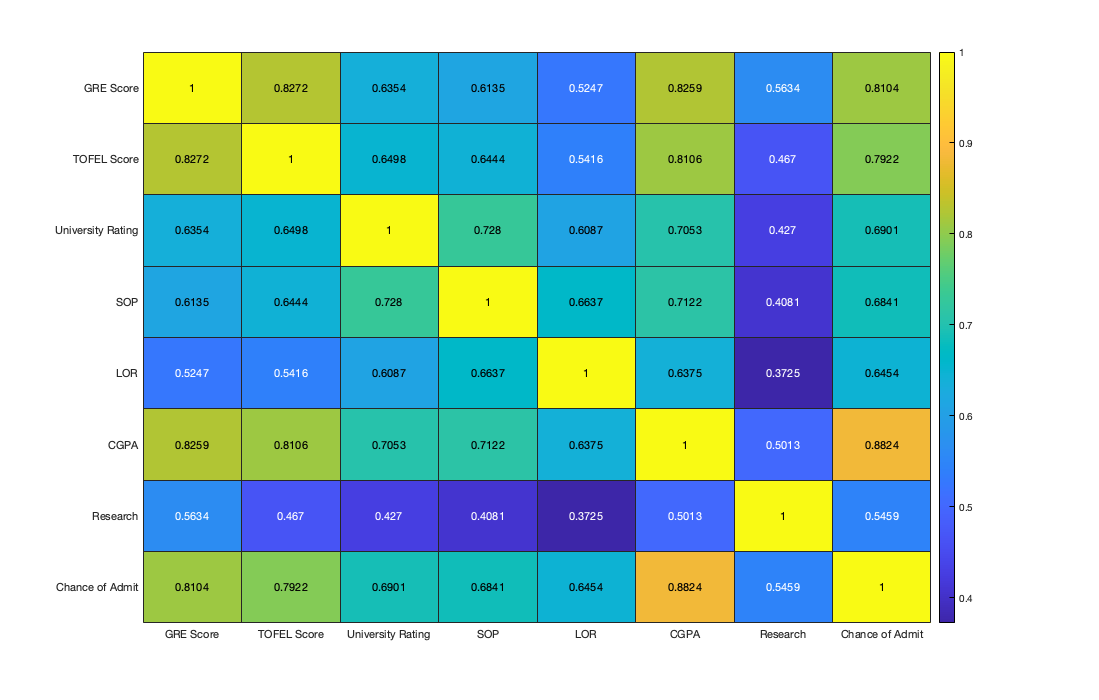
\includegraphics[scale=0.35]{images/heatmap.png}
\end{figure}
从上图我们可以发现录取几率和自变量GRE分数、CGPA、TOEFL成绩的相关性较高。同时CGPA、TOFEL分数、GRE分数之间的相关性也都很高。
\subsection{建立多元线性回归模型}
\subsubsection*{建立全模型}
首先,我们对所有预测变量进行回归,得到全模型的回归方程。再对回归方程做相关的显著性检验。

鉴于已有的 MATLAB 函数中对于线性回归的 regress 函数所能提供的输出过少,并没有相关的统计指标与统计检验,无法满足需求。因此,我单独编写了 myregression 函数,将相应的指标都进行了一定的计算,对于对应的检验同时输出了 p 值,以供判断。具体的代码如下:
\begin{lstlisting}
function [beta,r2,adjr2,F,Ftest,t,ttest,residuals] = myregression(x,y)
n = size(x,1);
m = size(x,2);
b = ones(n,1);
x = [b,x];
beta = (x'*x)\(x'*y);
ttest = zeros(1,m+1);
sst=(y-mean(y))'*(y-mean(y));
sse=(y-x*beta)'*(y-x*beta);
ssr=sst-sse;
F=(ssr/m)/(sse/(n-m-1));
r2=ssr/sst;
adjr2=1-(n-1)/(n-m-1)*(1-r2);
Ftest=1-fcdf(F,m,n-m-1);
c=diag(inv(x'*x));
t=zeros(1,m+1);
sigma=sqrt(sse/(n-m-1));
for i=1:m+1
t(i)=beta(i)/(sqrt(c(i))*sigma);
ttest(i)=2*(1-tcdf(abs(t(i)),n-m-1));
end
residuals = y-x*beta;
\end{lstlisting}

参数估计、t检验结果、$R^2$ 值和调整的 $R^2$ 值等各项统计指标汇总于下表
\begin{table}[H]
	\centering
	\caption{全模型各项指标汇总}
	\begin{tabular}{ccccccccc}
		\hline\hline
		    变量& Intercept& $x_1$    & $x_2$    & $x_3$   & $x_4$    & $x_5$    & $x_6$    & $x_7$  \\
		    \hline
	估计	&  -1.235102   &  0.001787   & 0.002581   &  0.005412   & 0.003872    &  0.016011   & 0.118506    &0.023749 \\
		t值& -12.010    &   3.618  & 3.005   & 1.447     &  0.858   & 3.927    &  12.423  &3.659 \\
		P值&  .000***   &.000***     &.002**    & .149    &.391     & .000***    &.000***   &.000*** \\
		\hline\hline
\multicolumn{4}{c}{$R^2$} & \multicolumn{4}{c}{调整$R^2$}& \\
\hline
		\multicolumn{4}{c}{0.8223}& \multicolumn{4}{c}{0.8198 
		}&\\
		\hline\hline
	\end{tabular}
\end{table}
通过上表数据我们可以发现回归方程整体效果良好,但存在参数并不显著。下面我们进行变量选择,我们将依次采用逐步回归、LASSO 回归和 Elastic Net。
\subsubsection*{变量选择1---逐步回归}
首先我们通过逐步回归进行变量选择,并指定模型选择标准为 AIC 准则。

我们选择 MATLAB 函数 stepwiselm 来实现该项功能,并选择 “Criterion” 为 “aic”,“Upper” 为 "linear",忽略交叉项的考虑。

选择的结果列于下表:
\begin{table}[H]
	\centering
	\caption{逐步回归子模型各项指标汇总}
	\label{tab4}
	\begin{tabular}{cccccccc}
		\hline\hline
		变量& Intercept& $x_1$    & $x_2$    & $x_3$   &   $x_5$    & $x_6$    & $x_7$ \\
		\hline
		估计	& -1.2462544    & 0.0017757   & 0.0026542   & 0.0065987    & 0.0170505   & 0.1199758    &  0.0238714  \\
		t值& -12.220     &    3.597  & 3.107   & 1.9    &  4.381   & 12.788     &  3.680    \\
		P值&  .000***
		&.000**   &.002**     &.058.    & .000***   &.000***     & .000***   \\
		\hline\hline
		\multicolumn{4}{c}{$R^2$} & \multicolumn{3}{c}{调整$R^2$}& \\
		\hline
		\multicolumn{4}{c}{ 0.8221}& \multicolumn{3}{c}{0.8199}&\\
		\hline\hline
	\end{tabular}
\end{table}
通过上表的各项指标,我们发现逐步回归建立的子模型删去了变量 SOP,整体的 $R^2$ 和调整后的 $R^2$ 基本没有太大改变,但相应的各预测变量的显著性得到了进一步的改进。

\subsubsection*{变量选择2---LASSO回归}
由于逐步回归的惩罚函数不连续,且每一次选择的跨度过大,所以下面我们尝试采用 LASSO 回归的稀疏性进行变量选择,并观察其选择结果。其中 $\lambda$ 的选择采用交叉验证(CV)。

采用CV交叉验证选取 $\lambda$ 值为 0.0000125(由于 CV 分组存在随机性,故可能每次运行结果不一致),此时各变量参数列于下表
\begin{table}[H]
	\centering
	\caption{LASSO回归变量参数}
	\label{tab4}
	\begin{tabular}{ccccccccc}
		\hline
		变量& Intercept& $x_1$    & $x_2$    & $x_3$& $x_4$ &   $x_5$    & $x_6$    & $x_7$ \\
		\hline
		估计	& -1.1054    & 0.001682   & 0.001876   & 0.002508    & 0.001178 &0.009416&0.121944&0.007376\\
		\hline
	\end{tabular}
\end{table}
下面我们给出CV验证下不同 $\lambda$ 的交叉验证误差图。
\begin{figure}[H]
\centering
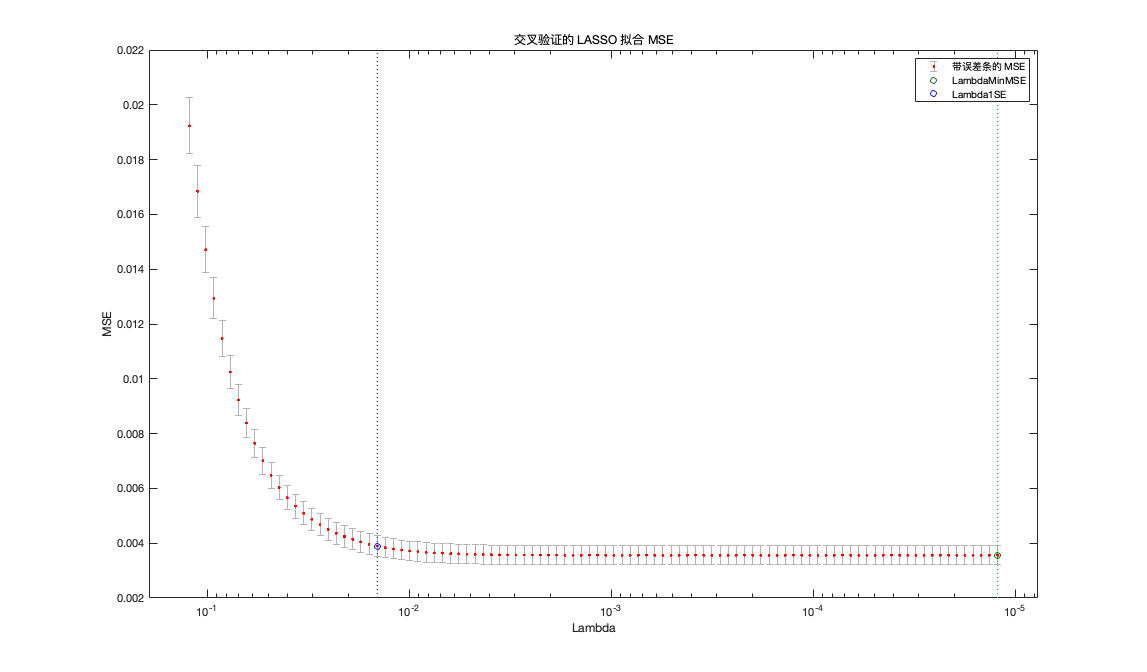
\includegraphics[scale=0.35]{images/LASSO2.png}
\end{figure}
综上所述,我们得到 LASSO 回归并没有删去任何变量,选择全模型。
\subsubsection*{变量选择3---Elastic Net}
由于 LASSO 回归的惩罚函数存在有偏性,下面我将尝试采用 Elastic Net 进行变量选择,其中 $\lambda$ 的选择采用交叉验证(CV)。

采用 CV 交叉验证选取 $\lambda$ 值为 0.0000163(由于 CV 分组存在随机性,故可能每次运行结果不一致),此时各变量参数列于下表
\begin{table}[H]
	\centering
	\caption{Elastic Net 变量参数}
	\label{tab4}
	\begin{tabular}{ccccccccc}
		\hline
		变量& Intercept& $x_1$    & $x_2$    & $x_3$& $x_4$ &   $x_5$    & $x_6$    & $x_7$ \\
		\hline
		估计	& -1.115540    &  0.001717   & 0.001995   & 0.002913    &  0.001662 &0.010131&0.119603&0.008938\\
		\hline
	\end{tabular}
\end{table}
下面我们给出 CV 验证下不同组别的交叉验证误差图。
\begin{figure}[H]
\centering
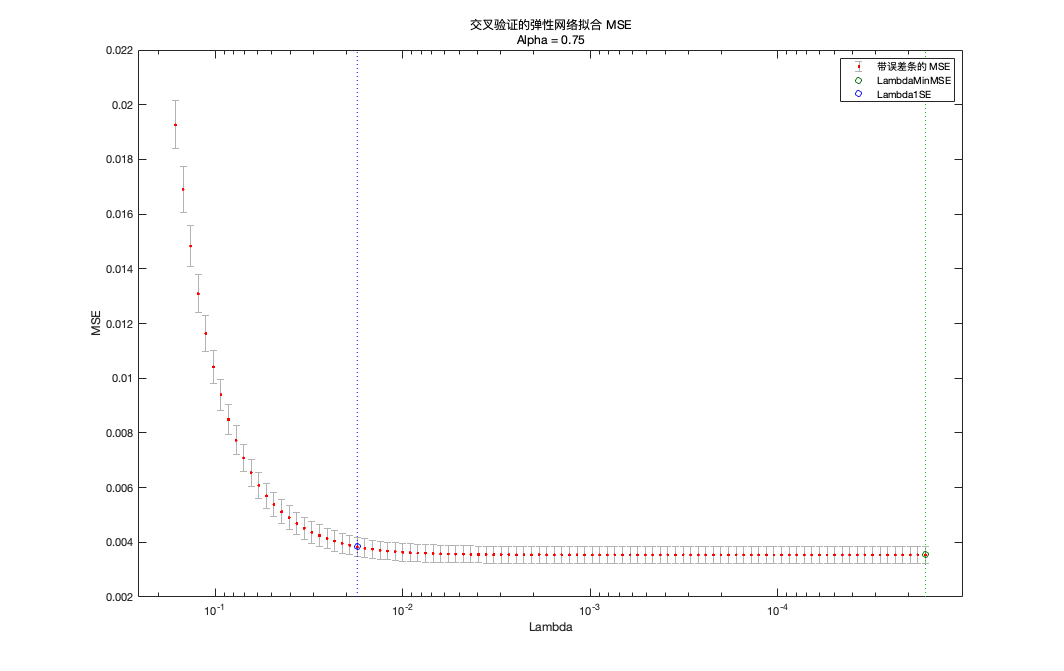
\includegraphics[scale=0.35]{images/Elastic2.png}
\end{figure}
综上所述,我们得到 Elastic Net 并没有删去任何变量,选择全模型。

我们通过结果发现这里 LASSO 和 Elastic Net 对变量的分离效果不是很好,综合上述三种方法得到的选择结果,我们最终选择子模型$\{x_1,x_2,x_3,x_5,x_6,x_7\}$。
\subsection{异方差的检验与处理}
首先,我们画出响应变量 Y 关于残差的散点图,通过图像进行初步判断。
\begin{figure}[H]
	\centering
	\caption{修正前残差散点图}
	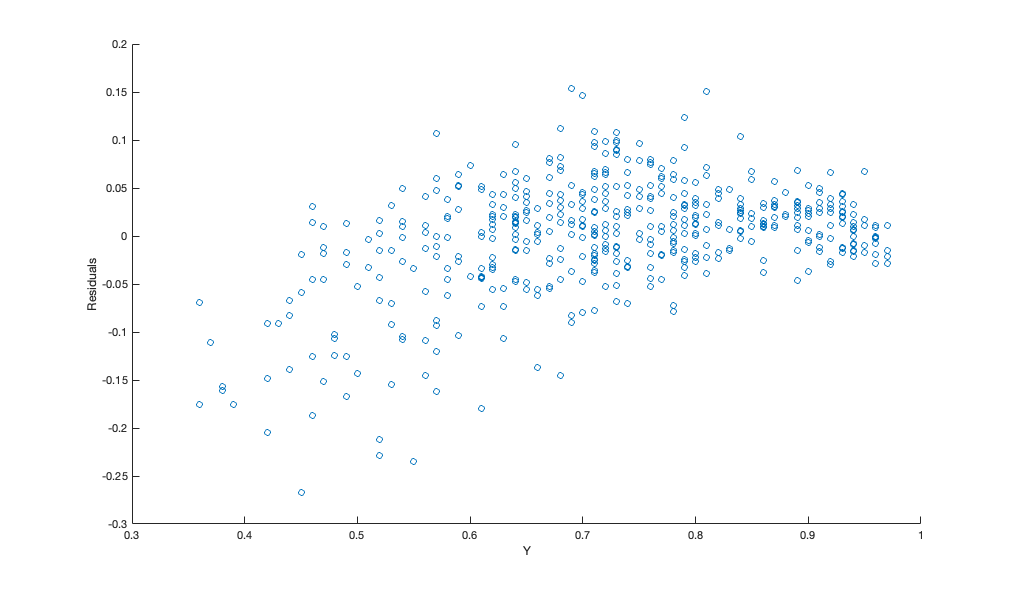
\includegraphics[scale=0.33]{images/residuals_inital.png}
\end{figure}
通过上图,我并不能准确判断回归方程是否存在异方差,需要进行进一步检验
\subsubsection*{异方差检验1---Spearman检验}
为了确定回归方程的异方差性,下面我们对各个预测变量做Spearman检验。

由于 MATLAB 函数中并没有相关检验的函数,因此我们编写了相应的检验函数 spearmantest,输入值为任意一个回归变量的观测样本向量和回归后的残差向量,输出值为 spearman 相关系数,对应检验的 t 值和检验 p 值。具体代码如下:
\begin{lstlisting}
function [rho,tvalue,pvalue] = spearmantest(x,residual)
n = size(x,1);
[rho,p] = corr(x,abs(residual),"type","Spearman");
tvalue = (sqrt(n-2)*rho)/sqrt(1-rho^2);
pvalue = 2*(1-tcdf(abs(tvalue),n-2));
end
\end{lstlisting}

检验的结果列于下表中
\begin{table}[H]
	\centering
	\caption{Spearman检验结果}
	\begin{tabular}{ccccccc}
		\hline
		变量& $x_1$    & $x_2$    & $x_3$   &   $x_5$    & $x_6$    & $x_7$\\
		\hline
		P值&0&0&0&0&0&0.001521\\
		rho&-0.316197&-0.2512531&-0.2112627&-0.2772145 &-0.3240891&-0.1418634\\
		\hline
	\end{tabular}
\end{table}

由此可见,各变量的 P 值均很低,存在强烈的异方差。

\subsubsection*{异方差检验2---white检验}
我们通过 white 检验,我们可以对回归方程整体的异方差性进行检验

由于 MATLAB 函数中并没有相关检验的函数,因此我们编写了相应的检验函数 whitetest,输入值为回归变量的观测样本矩阵和回归后的残差向量,输出值为 White 统计量和检验 p 值。具体代码如下:
\begin{lstlisting}
function [W,pvalue] = whitetest(x,residual)
n=size(x,1);
m=size(x,2);
res2 = residual.^2;
xtest =x;
for i =1:m
xtest = [xtest,x(:,i).^2];
end
[betat,r2t,adjr2t,Ft,Ftestt,tt,ttestt,residualst] = myregression(xtest,res2);
W=n*r2t;
pvalue = 1-chi2cdf(W,size(xtest,2));
end
\end{lstlisting}

检验结果如下:
\begin{center}
	\fcolorbox{black}{gray!10}{\parbox{.9\linewidth}{
W=34.8798, p-value =
0.0004894
	}}
\end{center}
white检验同样显示,回归方程存在异方差性。

\subsubsection*{异方差处理--------BOX-COX变换}
BOX-COX 变换是在 1964 年由 BOX 和 COX 提出的一种通过对因变量处理来消除异方差的方法,主要进行的变换为:
$$
y^{(\lambda)}=\left\{\begin{array}{cl}
	\dfrac{y^\lambda-1}{\lambda}&,\lambda\ne 0\\
	\ln y&,\lambda=0\\
\end{array}\right.
$$
其中 $\lambda$ 为待定系数。

此变换要求 $y$ 的各分量都大于 0。否则可先将因变量 $y$ 做一个平移变换,使得平移后各分量均大于0,再进行 BOX-COX 变换。从而我们得到推广的 BOX-COX 变换:
$$
y^{(\lambda)}=\left\{\begin{array}{cl}
	\dfrac{(y+a)^\lambda-1}{\lambda}&,\lambda\ne 0\\
	\ln (y+a)&,\lambda=0\\
\end{array}\right.
$$

很显然,在不同的 $\lambda$ 下,因变量 $y$ 所作的变换是不一样的,产生的效果也是不一样的。为了消除异方差,我们希望寻找到合适的 $\lambda$,使得便后有:
$$
y^{(\lambda)}=\begin{pmatrix}
	y_1^{(\lambda)}\\
	y_2^{(\lambda)}\\
	\vdots\\
	y_n^{(\lambda)}
\end{pmatrix}\sim N(X\beta,\sigma^2I)
$$

事实上,由此我们可以发现,BOX-COX 变换不仅可以处理异方差性问题,还能处理自相关、误差非正态、回归函数非线性等问题。

寻找合适的 $\lambda$ 的方法有很多,我们可以通过计算 $\lambda$ 的对数极大似然估计得到。$\lambda$ 的极大似然估计:
$$
L_{\max}(\lambda)=(2\pi e\hat{\sigma}_\lambda^2)^{-\frac{n}{2}}|J|
$$
式中,$\hat{\sigma}^2_\lambda=\dfrac{1}{n}SSE(\lambda,y^{(\lambda)}),|J|=\prod\limits_{i=1}^ny^{(\lambda)}$

令 $z^{(\lambda)}=\dfrac{y^{(\lambda)}}{|J|}$,对 $L_{\max}$取对数并忽略与 $\lambda$ 无关的常数项,可得:
$$
\ln L_{\max}(\lambda)=-\dfrac{n}{2}\ln SSE(\lambda,z^{(\lambda)})
$$

此时只需取使 $SSE(\lambda,z^{(\lambda)})$ 最小的 $\lambda$ 即可。但在实际情况中,其解析解一般无法得到,我们可以通过大量 $\lambda$ 值计算,得到近似最优解。

在这里我们从-5到5以步长为0.1依次取$\lambda$的取值进行回归,通过最大对数似然值来选取最终的$\lambda$。

在这里我们编写了一个在给定 $\lambda$ 下计算 SSE 值大小的函数,名称为 bocc,具体代码如下:
\begin{lstlisting}
function SSE=bocc(X,Y,lambda)
H=X*inv(X'*X)*X';
n=length(Y);
switch lambda
case 0
z=log(Y)*prod(Y)^(1/n);
otherwise
z=(Y.^lambda-1)/lambda/(prod(Y)^((lambda-1)/n));
end
SSE=z'*(eye(n)-H)*z;
end
\end{lstlisting}

各$\lambda$下的极大似然图如下所示
\begin{figure}[H]
	\centering
	\caption{BOX-COX变换下极大似然值}
	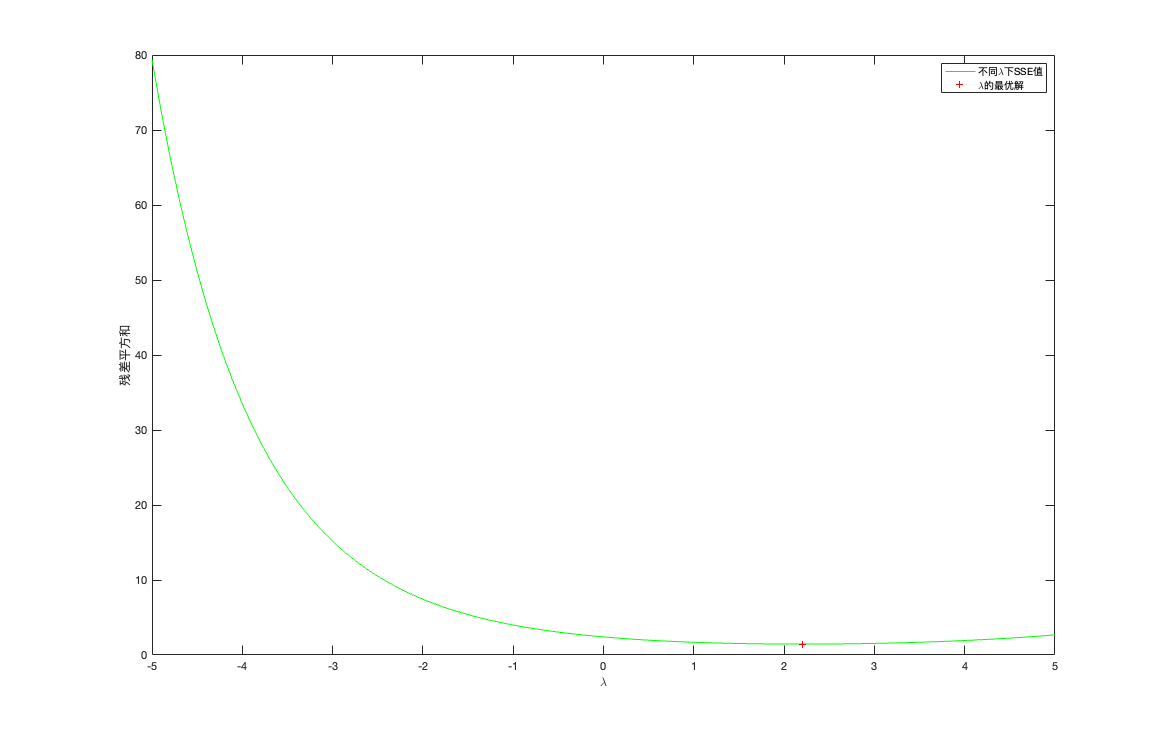
\includegraphics[scale=0.35]{images/box_cox_plot.png}
\end{figure}
$\lambda$最终取值为2.2,经过BOX-COX变换后,重新进行线性回归。我们将参数估计、t检验结果、$R^2$值和调整的$R^2$值汇总于下表:
\begin{table}[H]
	\centering
	\caption{BOX-COX变换后回归方程各项指标汇总}
	\begin{tabular}{cccccccc}
		\hline\hline
		变量& Intercept& $x_1$    & $x_2$    & $x_3$   &   $x_5$    & $x_6$    & $x_7$  \\
		\hline
		估计	& -1.5480818   &  0.0011814  & 0.0021030   & 0.0069611   & 0.0098556 & 0.0771804   &0.0167611\\
		t值& -24.758    &   3.903  & 4.015   & 3.268     &  4.130  &  13.417   &  4.214  \\
		P值&  .000***
		&.000***  &.000***     &.001**    & .000***   &.000***     & .000***  \\
		\hline\hline
		\multicolumn{4}{c}{$R^2$} & \multicolumn{4}{c}{调整$R^2$} \\
		\hline
		\multicolumn{4}{c}{0.8501}& \multicolumn{4}{c}{0.8483}\\
		\hline\hline
	\end{tabular}
\end{table}
经过变换后可以发现,P 值,$R^2$和调整的$R^2$均有明显的提高,回归方程的显著性有一定的提升,并且所有系数均通过了t检验。

我们重新再画出残差的散点图:

\begin{figure}[H]
	\centering
	\caption{BOX-COX变换后的残差散点图}
	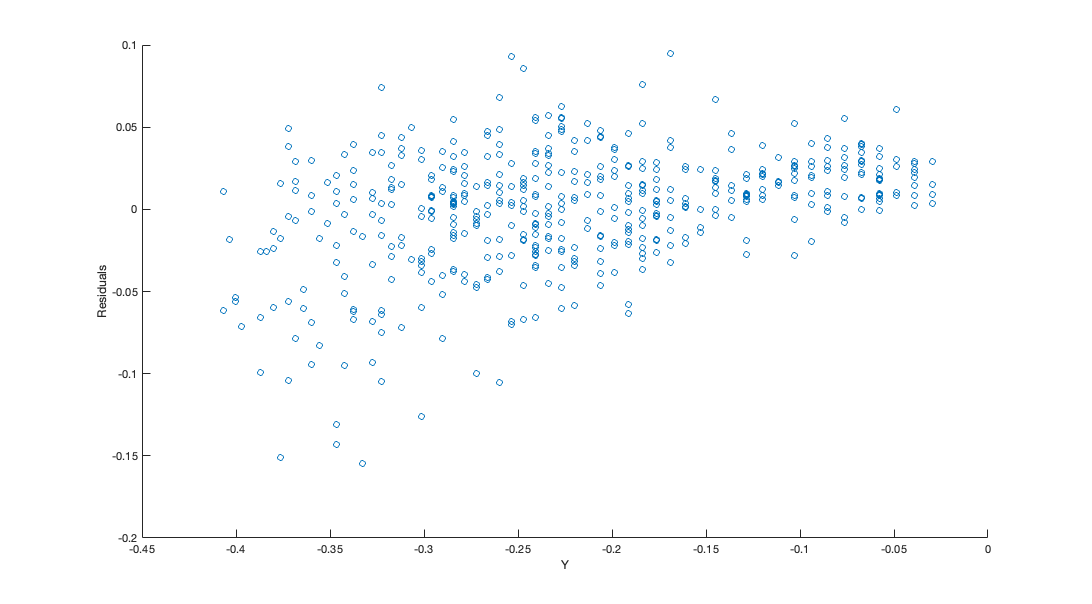
\includegraphics[scale=0.35]{images/box_cox_residuals.png}
\end{figure}

可以发现,残差有显著的减小。为了进一步地确定,我们再对各变量进行Spearman检验,检验结果列于下表
\begin{table}[H]
	\centering
	\caption{Spearman检验结果}
	\begin{tabular}{ccccccc}
		\hline
		变量& $x_1$    & $x_2$    & $x_3$   &   $x_5$    & $x_6$    & $x_7$\\
		\hline
		秩S&20367287&20338509&20547614&20806322&20308580&20533394\\
		P值&0.9193&0.8945&0.9246&0.707&0.8689&0.9369\\
		rho&0.004555572&0.005962061&-0.004257869&-0.01690215 &0.007424821&-0.003562844\\
		\hline
	\end{tabular}
\end{table}
再进行 white 检验,检验结果如下文本框
\begin{center}
	\fcolorbox{black}{gray!10}{\parbox{.9\linewidth}{
studentized Breusch-Pagan test

W = 20.6335,  p-value = 0.0560
	}}
\end{center}
通过上面两表中的数据,可以肯定,异方差已消除。
\subsection{自相关的检验与处理}
\subsubsection*{自相关检验---DW检验}
首先,我们画出残差$e_t$与$e_{t-1}$的散点图,通过图形来初步判断自相关性。散点图如下:
\begin{figure}[H]
	\centering
	\caption{残差时序图}
	\label{gra.15}
	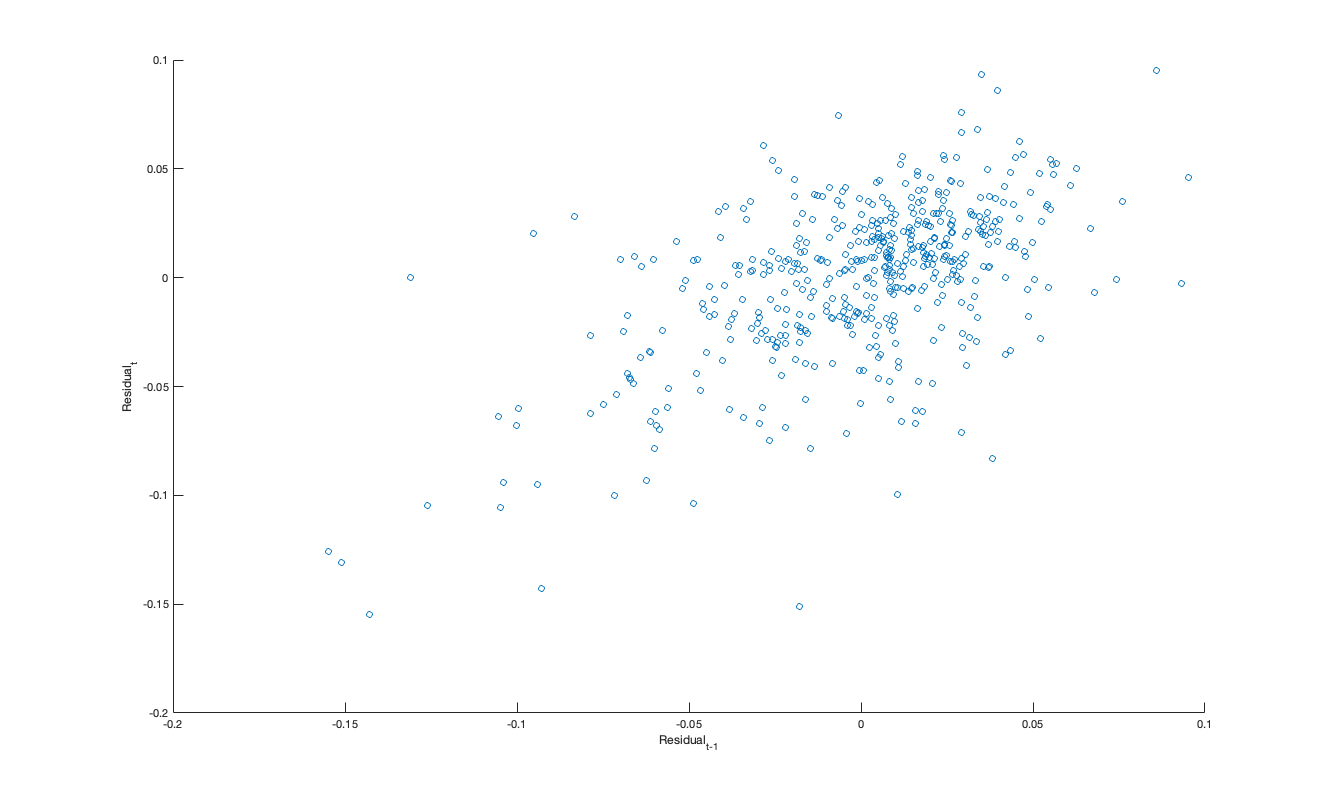
\includegraphics[scale=0.3]{images/residuals_sequence.png}
\end{figure}
通过图形,我们可以初步判断回归方程存在一定的自相关性。为了进一步的确定,我们下面对回归模型进行 DW 检验。

由于 MATLAB 并没有相关的计算函数,因此我们编写了 dwtest 函数,输入值为残差向量,输出值为 DW 值和相关系数估计值 $\hat{\rho}$

检验结果列于下表:
\begin{table}[H]
	\centering
	\caption{DW检验检验结果}
	\begin{tabular}{cccc}
		\hline
		D.W.值&P值&$D_L$&$D_U$\\
		\hline
		0.8723&0.000&1.70&1.83\\
		\hline
	\end{tabular}
\end{table}
由于$0\le D.W.\le D_L$,故回归方程的误差项之间存在正自相关性。
\subsubsection*{自相关的处理---迭代法}
我们通过图\ref{gra.15}可以初步判断,残差项存在一阶自回归形式,故我们采用迭代法进行处理。

对于一元回归方程而言,我们设一元线性回归模型的误差项存在一阶自相关性,即:
$$
\begin{array}{c}
y_t=\beta_0+\beta_1x_t+\varepsilon_t\\
\varepsilon_t=\rho\varepsilon_{t-1}+\mu_t
\end{array}
$$
其中 $\mu_t$ 满足 $Gauss-Markov$ 条件,即:
$$
\left\{\begin{array}{ll}
    E(\mu_t)=0 & t=1,2\cdots,n \\
     cov(\mu_t,\mu_s)=\left\{\begin{array}{ll}
         \sigma^2 & t=s \\
          0&t\ne s 
     \end{array}\right.& t,s=1,2,\cdots,n
\end{array}\right.
$$

通过上述条件,我们可以作如下变形:
$$
(y_t-\rho y_{t-1})=(\beta_0-\rho\beta_0)+\beta_1(x_t-\rho x_{t-1})+(\varepsilon_t-\rho\varepsilon_{t-1})
$$
下面我们令:
$$
\begin{array}{c}
     y'_t=y_t-\rho y_{t-1} \\
     x'_t=x_t-\rho x_{t-1}\\
     \beta_0'=\beta_0-\rho\beta_0\\
\end{array}
$$
从而获得新的回归方程如下:
$$
y'_t=\beta_0'+\beta_1x'_t+\mu_t
$$

很容易发现,获得的新的回归方程满足基本假设。在一般情况下,对于迭代法中的自相关系数 $\rho$,我们用 $\hat{\rho}=1-\dfrac{1}{2}\mathrm{DW}$ 来估计。

对于现在的多元情况,我们可以类似一元的情形进行处理。在这里,我们取$\hat{\rho}=1-\dfrac{1}{2}\mathrm{DW}=0.5638$ ,迭代后重新进行线性回归,我们将参数估计、t检验结果、$R^2$值和调整的$R^2$值汇总于下表:
\begin{table}[H]
	\centering
	\caption{迭代后回归方程各项指标汇总}
	\begin{tabular}{cccccccc}
		\hline\hline
		变量& Intercept& $x_1$    & $x_2$    & $x_3$   &   $x_5$    & $x_6$    & $x_7$  \\
		\hline
		估计	& -0.655759   &  0.001134  & 0.002534   & 0.005213   & 0.009079 & 0.069185   &0.018304\\
		t值& -29.684    &   4.744 &6.021   & 2.828     &  4.847   &  14.023   &  6.176  \\
		P值&  .000***
		&.000***  &.000***     &.006**    & .000***   &.000***     & .000***  \\
		\hline\hline
		\multicolumn{4}{c}{$R^2$} & \multicolumn{4}{c}{调整$R^2$} \\
		\hline
		\multicolumn{4}{c}{0.8351}& \multicolumn{4}{c}{0.8331}\\
		\hline\hline
	\end{tabular}
\end{table}

对于新得到的方程,我们重新画出残差时序图
\begin{figure}[H]
	\centering
	\caption{残差时序图}
	\label{gra.15}
	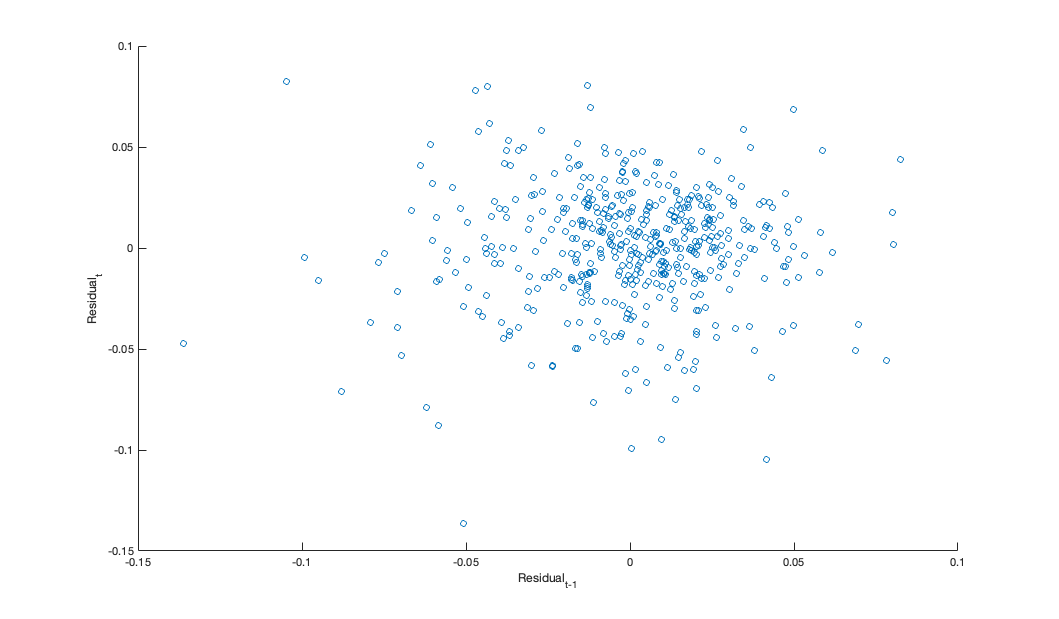
\includegraphics[scale=0.35]{images/residuals_interation.png}
\end{figure}
重新进行DW检验,检验结果列于下表:
\begin{table}[H]
\centering
\caption{D.W.检验结果}
\begin{tabular}{cccc}
		\hline
		D.W.值&P值&$D_L$&$D_U$\\
		\hline
		1.9717&0.3822&1.70&1.83\\
		\hline
	\end{tabular}
\end{table}
此时已通过DW检验,方程的共线性已消除。
\subsection{共线性检验与处理}
\subsubsection*{共线性检验--------VIF与条件数}
最后我们需要对得到的回归模型做共线性检验。我们首先计算各自变量的方差膨胀因子(VIF)。

由于 MATLAB并没有提供相关的计算函数,因此我们编写了 vif 函数来计算。该函数的输入值为回归变量的样本观测矩阵,输出为每个回归变量的方差膨胀因子。具体的代码如下:
\begin{lstlisting}
function [diagvalue] = vif(x)
x = corr(x,"type","Pearson");
diagvalue = diag(inv(x));
end
\end{lstlisting}
利用函数的计算结果如下表所示。
\begin{table}[H]
	\centering
	\caption{各自变量的VIF值}
	\begin{tabular}{ccccccc}
		\hline
		变量& $x_1$    & $x_2$    & $x_3$  &   $x_5$    & $x_6$    & $x_7$  \\
		\hline
		VIF&3.31510& 2.94016&1.75433&1.32270&3.23408&1.26914\\
		\hline
	\end{tabular}
\end{table}
由上表结果,我们发现回归方程不存在共线性。下面,我们再计算其条件数 k,进一步确认结果。

由于条件数的计算 MATLAB 并没有提供相应的函数,因此我们编写了对应的计算函数 condvaluecal。其中输入值为回归变量的样本观测矩阵,输出为每个回归变量的条件数。具体的代码如下:
\begin{lstlisting}
function [condvalue] = condvaluecal(x)
x = corr(x,type="Pearson");
eigvalue = eig(x);
eigmax = max(eigvalue);
condvalue = sqrt(eigmax./eigvalue);
end
\end{lstlisting}

计算得条件数如下表
\begin{table}[H]
	\centering
	\caption{各自变量的条件数}
	\begin{tabular}{ccccccc}
		\hline
		变量& $x_1$    & $x_2$    & $x_3$  &   $x_5$    & $x_6$    & $x_7$  \\
		\hline
		k&1& 4.172&3.748&2.699&2.223&2.170\\
		\hline
	\end{tabular}
\end{table}
由上表结果,我

由此可以确定,方程不存在共线性。

\section{模型分析与评价}
\subsection{模型分析}
通过上述变换后我们最终得到了如下回归方程:
$$
\left\{\begin{array}{l}
z'=--0.65575+0.001134x_1'+0.002534x_2'+0.005213x_3'+0.009079x_5'+0.069185x_6'+0.018304x_7'\\
z'=\dfrac{z^\lambda-1}{\lambda}\\
\lambda=2.2
\end{array}\right.
$$
下面我们进行回归诊断,主要为残差分析与影响分析,用来检验回归方程是否存在大量异常值点。

异常值通常分为三类,具体定义如下:
\begin{itemize}
    \item[-]离群点(Outlier):通常指残差非常大的点。模型预测的 $y$ 值与真实的 $y$ 值相差很大,是关于 $y$ 异常的点。
    \item[-]高杠杆值点(High-leverage point):一般是指关于 $x$ 异常的点,与响应变量 $y$ 没有直接关系。
    \item[-]强影响点(Influnce point):关于模型异常的点,不一定关于 $x$ 或关于 $y$ 异常。
\end{itemize}
-离群点(Outlier)

在残差分析中,我们一般认为残差超过 $\pm3\hat{\sigma}$ 的点为异常值点。通常使用的残差主要为:

\begin{itemize}
    \item [-] 普通残差:$e_i=y_i-\hat{y}_i$
    \item [-] 标准化残差:$ZRE_i=\dfrac{e_i}{\hat{\sigma}}$
    \item [-] 学生化残差:$SRE_i=\dfrac{e_i}{\hat{\sigma}\sqrt{1-h_{ii}}}$,其中 $h_{ii}$ 为帽子矩阵 $H=X(X^TX)'X^T$ 对于的主对角线元素。
\end{itemize}

然而对于离群点而言,标准残差、学生化残差和普通残差都不在适用,因为离群点会把回归线拉向自身,从而使其本身的残差减小,其余观测的残差增大,回归的标准差 $\hat{\sigma}$ 也相应增大。此时我们采用删除残差来判断。

删除残差构造的主要思想:在计算第 $i$ 个观测值的残差时,我们使用剩余的 $n-1$ 个观测进行线性回归拟合,此时得到的拟合值 $\hat{y}_{(i)}$ 与第 $i$ 个观测值无关,由此定义其删除残差为
$$
e_{(i)}=y_i-\hat{y}_{(i)}=\dfrac{e_i}{1-h_{ii}}
$$
进一步,此时对应的删除学生残差为:
$$
SRE_{(i)}=SRE_i\cdot(\dfrac{n-p-2}{n-p-1-SRE_i^2})^{\frac{1}{2}}
$$

一般情况下,当 $|SRE_{(i)}|>3$ 时,我们判定该点为离群点。

-高杠杆值点(High-leverage point)
在多元线性回归中,$D(e_i)=(1-h_{ii})\sigma^2$,其中 $h_{ii}$ 为帽子矩阵中主对角线的第 $i$ 个元素,它是调节 $e_i$ 方差大小的杠杆,故我们常称 $h_{ii}$ 为第 $i$ 个观测的杠杆值。同时,$h_{ii}$ 也代表了自变量的第 $i$ 次观测与自变量平均值之间距离的远近。具有较大杠杆值的观测点远离样本中心,能够把回归拉向自身。

一般情况下,我们用杠杆值的平均值作为评判标准,来区分高杠杆值点。由于 $tr(H)=\sum\limits_{i=1}^nh_{ii}=p+1$,所以:
$$
\bar{h}=\dfrac{1}{n}\sum\limits_{i=1}^nh_{ii}=\dfrac{p+1}{n}
$$
当一个观测点的杠杆值 $h_{ii}$ 大于 2 倍或 3 倍的 $\bar{h}$ 时,我们可以认为该点为高杠杆值点。

-强影响点(Influnce point)
对于强影响点,我们一般采用库克距离来判别,库克距离的计算公式为:
$$
D_i=\dfrac{\sum\limits_{j=1}^n(\hat{y}_j-\hat{y}_{j(i)})^2}{(p+1)\hat{\sigma}^2}=\dfrac{e_i^2}{(p+1)\hat{\sigma}^2}\cdot\dfrac{h_{ii}}{(1-h_{ii})^2}
$$

通过定义式,我们可以发现库克距离是反映了杠杆值 $h_{ii}$ 和残差 $e_i$ 的综合效应。对于强影响点,我们粗略的判断准则如下:
\begin{itemize}
	\item 当 $D_i<0.5$ 时,认为该点不是异常值点。
	\item 当 $D_i>1$ 时,认为该点为异常值点。
\end{itemize}

下面我们画出学生化残差图、cook距离图与杠杆值倍数图。
\begin{figure}[H]
\centering
\caption{学生化残差}
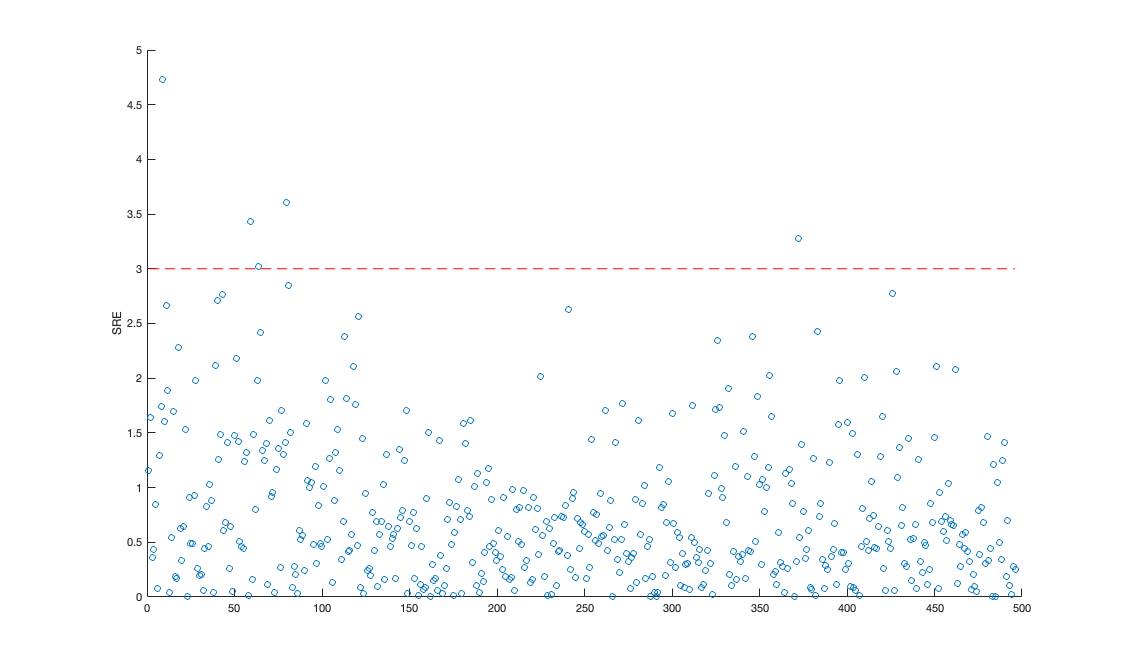
\includegraphics[scale=0.33]{images/stu_res.png}
\end{figure}
\begin{figure}[H]
\centering
\caption{Cook-Distance}
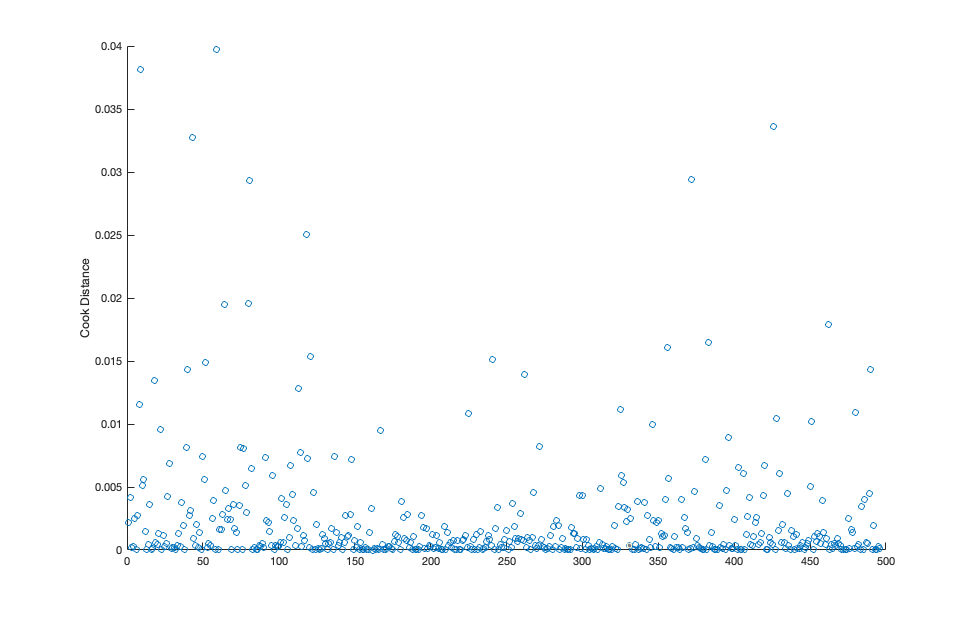
\includegraphics[scale=0.35]{images/cook.png}
\end{figure}
\begin{figure}[H]
	\centering
	\caption{High-leverage}
	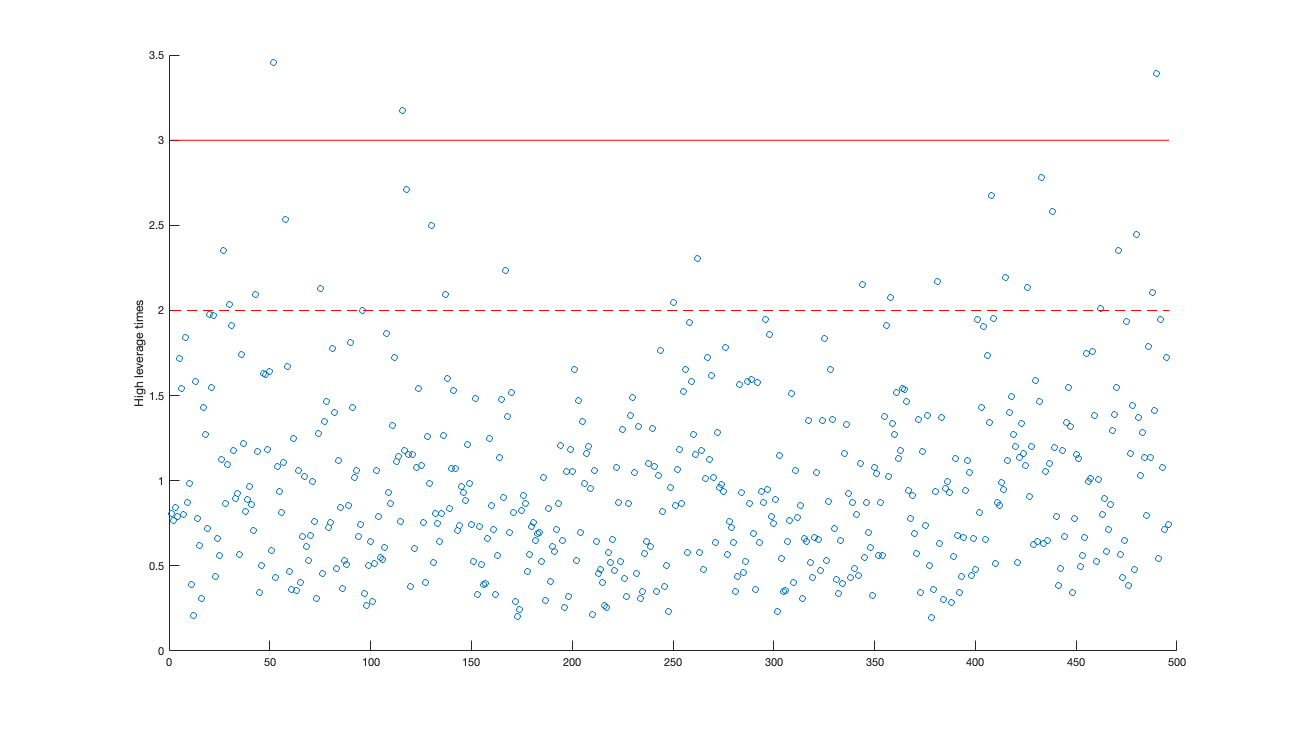
\includegraphics[scale=0.31]{images/hlt.png}
\end{figure}
从上面三张图可以看出,所得回归方程的学生化残差基本落在[-2,2]之间,只有少量点落在-4以外,Cook距离均在0.04以下,没有强影响点存在,但存在部分的高杠杆值点。
\subsection{模型解释}
从所得回归方程我们可以发现,大学的录取率和个人推荐信的好坏并没有很大的关系,而和本科GPA与是否具有科研经历具有密切关系。从而,对于印度的本科生而言,需要更加注重GPA和科研方面。
\subsection{模型优缺点}
\subsubsection*{优点}
\begin{itemize}
\item [1] 采用线性回归模型,通俗易懂,便于理解。可以很好的了解各变量对因变量的影响程度。
\item [2] 回归拟合效果好,显著很高。
\end{itemize}
\subsubsection*{缺点}
\begin{itemize}
\item [1] 存在一些离群点和高杠杆值点未处理。
\item [2] 数据没有划分出训练集与测试集,对于所得方程的应用效果有待检验。
\end{itemize}
\addcontentsline{toc}{section}{Reference}
\begin{thebibliography}{99}  
	\bibitem{ref1}何晓群, 刘文卿. 应用回归分析[M]. 中国人民大学出版社, 2001.  
	\bibitem{ref2}Mazu, Michael J . Regression Analysis by Example[J]. Technometrics, 1977, 35(1):86-87.
	\bibitem{ref3}Mohan S Acharya, Asfia Armaan, Aneeta S Antony : A Comparison of Regression Models for Prediction of Graduate Admissions, IEEE International Conference on Computational Intelligence in Data Science 2019
\end{thebibliography}
\newpage
\addcontentsline{toc}{section}{Appendix}
\begin{appendix}
	\section{原始数据}
	\begin{longtable}[H]{|c|c|c|c|c|c|c|c|c|}
	\hline
	Serial No. & GRE & TOEFL & University Rating & SOP & LOR & CGPA & Research & Chance of Admit\\ \hline
	1          & 337& 118 & 4 & 4.5 & 4.5 & 9.65 & 1        & 0.92            \\ \hline
	2          & 324& 107  & 4 & 4   & 4.5 & 8.87 & 1        & 0.76            \\ \hline
	3          & 316  & 104 & 3   & 3   & 3.5 & 8    & 1        & 0.72            \\ \hline
	4          & 322   & 110  & 3   & 3.5 & 2.5 & 8.67 & 1        & 0.8             \\ \hline
	5          & 314       & 103  & 2& 2   & 3   & 8.21 & 0        & 0.65            \\ \hline
	6          & 330       & 115   & 5 & 4.5 & 3   & 9.34 & 1        & 0.9             \\ \hline
	7          & 321       & 109  & 3   & 3   & 4   & 8.2  & 1        & 0.75            \\ \hline
	8          & 308       & 101   & 2 & 3   & 4   & 7.9  & 0        & 0.68            \\ \hline
	9          & 302       & 102 & 1 & 2   & 1.5 & 8    & 0        & 0.5             \\ \hline
	10         & 323       & 108  & 3   & 3.5 & 3   & 8.6  & 0        & 0.45            \\ \hline
	11         & 325       & 106  & 3   & 3.5 & 4   & 8.4  & 1        & 0.52            \\ \hline
	12         & 327       & 111  & 4 & 4   & 4.5 & 9    & 1        & 0.84            \\ \hline
	13         & 328       & 112         & 4   & 4   & 4.5 & 9.1  & 1        & 0.78            \\ \hline
	14         & 307       & 109         & 3  & 4   & 3   & 8    & 1        & 0.62            \\ \hline
	15         & 311       & 104         & 3  & 3.5 & 2   & 8.2  & 1        & 0.61            \\ \hline
	16         & 314       & 105         & 3  & 3.5 & 2.5 & 8.3  & 0        & 0.54            \\ \hline
	17         & 317       & 107         & 3  & 4   & 3   & 8.7  & 0        & 0.66            \\ \hline
	18         & 319       & 106         & 3  & 4   & 3   & 8    & 1        & 0.65            \\ \hline
	19         & 318       & 110         & 3   & 4   & 3   & 8.8  & 0        & 0.63            \\ \hline
	20         & 303       & 102         & 3  & 3.5 & 3   & 8.5  & 0        & 0.62            \\ \hline
	21         & 312       & 107         & 3 & 3   & 2   & 7.9  & 1        & 0.64            \\ \hline
	22         & 325       & 114         & 4    & 3   & 2   & 8.4  & 0        & 0.7             \\ \hline
	23         & 328       & 116         & 5  & 5   & 5   & 9.5  & 1        & 0.94            \\ \hline
	24         & 334       & 119         & 5   & 5   & 4.5 & 9.7  & 1        & 0.95            \\ \hline
	25         & 336       & 119         & 5  & 4   & 3.5 & 9.8  & 1        & 0.97            \\ \hline
	26         & 340       & 120         & 5   & 4.5 & 4.5 & 9.6  & 1        & 0.94            \\ \hline
	27         & 322       & 109         & 5  & 4.5 & 3.5 & 8.8  & 0        & 0.76            \\ \hline
	28         & 298       & 98          & 2   & 1.5 & 2.5 & 7.5  & 1        & 0.44            \\ \hline
	29         & 295       & 93          & 1   & 2   & 2   & 7.2  & 0        & 0.46            \\ \hline
	30         & 310       & 99          & 2  & 1.5 & 2   & 7.3  & 0        & 0.54            \\ \hline
	31         & 300       & 97          & 2   & 3   & 3   & 8.1  & 1        & 0.65            \\ \hline
	32         & 327       & 103         & 3   & 4   & 4   & 8.3  & 1        & 0.74            \\ \hline
	33         & 338       & 118         & 4  & 3   & 4.5 & 9.4  & 1        & 0.91            \\ \hline
	34         & 340       & 114         & 5   & 4   & 4   & 9.6  & 1        & 0.9             \\ \hline
	35         & 331       & 112         & 5  & 4   & 5   & 9.8  & 1        & 0.94            \\ \hline
	36         & 320       & 110         & 5  & 5   & 5   & 9.2  & 1        & 0.88            \\ \hline
	37         & 299       & 106         & 2  & 4   & 4   & 8.4  & 0        & 0.64            \\ \hline
	38         & 300       & 105         & 1 & 1   & 2   & 7.8  & 0        & 0.58            \\ \hline
	39         & 304       & 105         & 1  & 3   & 1.5 & 7.5  & 0        & 0.52            \\ \hline
	40         & 307       & 108         & 2   & 4   & 3.5 & 7.7  & 0        & 0.48            \\ \hline
	41         & 308       & 110         & 3& 3.5 & 3   & 8    & 1        & 0.46            \\ \hline
	42         & 316       & 105         & 2 & 2.5 & 2.5 & 8.2  & 1        & 0.49            \\ \hline
	43         & 313       & 107         & 2 & 2.5 & 2   & 8.5  & 1        & 0.53            \\ \hline
	44         & 332       & 117         & 4  & 4.5 & 4   & 9.1  & 0        & 0.87            \\ \hline
	45         & 326       & 113         & 5  & 4.5 & 4   & 9.4  & 1        & 0.91            \\ \hline
	46         & 322       & 110         & 5  & 5   & 4   & 9.1  & 1        & 0.88            \\ \hline
	47         & 329       & 114         & 5   & 4   & 5   & 9.3  & 1        & 0.86            \\ \hline
	48         & 339       & 119         & 5  & 4.5 & 4   & 9.7  & 0        & 0.89            \\ \hline
	49         & 321       & 110         & 3   & 3.5 & 5   & 8.85 & 1        & 0.82            \\ \hline
	50         & 327       & 111         & 4  & 3   & 4   & 8.4  & 1        & 0.78            \\ \hline
	51         & 313       & 98          & 3  & 2.5 & 4.5 & 8.3  & 1        & 0.76            \\ \hline
	52         & 312       & 100         & 2  & 1.5 & 3.5 & 7.9  & 1        & 0.56            \\ \hline
	53         & 334       & 116         & 4   & 4   & 3   & 8    & 1        & 0.78            \\ \hline
	54         & 324       & 112         & 4& 4   & 2.5 & 8.1  & 1        & 0.72            \\ \hline
	55         & 322       & 110         & 3  & 3   & 3.5 & 8    & 0        & 0.7             \\ \hline
	56         & 320       & 103         & 3   & 3   & 3   & 7.7  & 0        & 0.64            \\ \hline
	57         & 316       & 102         & 3 & 2   & 3   & 7.4  & 0        & 0.64            \\ \hline
	58         & 298       & 99          & 2   & 4   & 2   & 7.6  & 0        & 0.46            \\ \hline
	59         & 300       & 99          & 1                 & 3   & 2   & 6.8  & 1        & 0.36            \\ \hline
	60         & 311       & 104         & 2                 & 2   & 2   & 8.3  & 0        & 0.42            \\ \hline
	61         & 309       & 100         & 2                 & 3   & 3   & 8.1  & 0        & 0.48            \\ \hline
	62         & 307       & 101         & 3                 & 4   & 3   & 8.2  & 0        & 0.47            \\ \hline
	63         & 304       & 105         & 2                 & 3   & 3   & 8.2  & 1        & 0.54            \\ \hline
	64         & 315       & 107         & 2                 & 4   & 3   & 8.5  & 1        & 0.56            \\ \hline
	65         & 325       & 111         & 3                 & 3   & 3.5 & 8.7  & 0        & 0.52            \\ \hline
	66         & 325       & 112         & 4                 & 3.5 & 3.5 & 8.92 & 0        & 0.55            \\ \hline
	67         & 327       & 114         & 3                 & 3   & 3   & 9.02 & 0        & 0.61            \\ \hline
	68         & 316       & 107         & 2                 & 3.5 & 3.5 & 8.64 & 1        & 0.57            \\ \hline
	69         & 318       & 109         & 3                 & 3.5 & 4   & 9.22 & 1        & 0.68            \\ \hline
	70         & 328       & 115         & 4                 & 4.5 & 4   & 9.16 & 1        & 0.78            \\ \hline
	71         & 332       & 118         & 5                 & 5   & 5   & 9.64 & 1        & 0.94            \\ \hline
	72         & 336       & 112         & 5                 & 5   & 5   & 9.76 & 1        & 0.96            \\ \hline
	73         & 321       & 111         & 5                 & 5   & 5   & 9.45 & 1        & 0.93            \\ \hline
	74         & 314       & 108         & 4                 & 4.5 & 4   & 9.04 & 1        & 0.84            \\ \hline
	75         & 314       & 106         & 3                 & 3   & 5   & 8.9  & 0        & 0.74            \\ \hline
	76         & 329       & 114         & 2                 & 2   & 4   & 8.56 & 1        & 0.72            \\ \hline
	77         & 327       & 112         & 3                 & 3   & 3   & 8.72 & 1        & 0.74            \\ \hline
	78         & 301       & 99          & 2                 & 3   & 2   & 8.22 & 0        & 0.64            \\ \hline
	79         & 296       & 95          & 2                 & 3   & 2   & 7.54 & 1        & 0.44            \\ \hline
	80         & 294       & 93          & 1                 & 1.5 & 2   & 7.36 & 0        & 0.46            \\ \hline
	81         & 312       & 105         & 3                 & 2   & 3   & 8.02 & 1        & 0.5             \\ \hline
	82         & 340       & 120         & 4                 & 5   & 5   & 9.5  & 1        & 0.96            \\ \hline
	83         & 320       & 110         & 5                 & 5   & 4.5 & 9.22 & 1        & 0.92            \\ \hline
	84         & 322       & 115         & 5                 & 4   & 4.5 & 9.36 & 1        & 0.92            \\ \hline
	85         & 340       & 115         & 5                 & 4.5 & 4.5 & 9.45 & 1        & 0.94            \\ \hline
	86         & 319       & 103         & 4                 & 4.5 & 3.5 & 8.66 & 0        & 0.76            \\ \hline
	87         & 315       & 106         & 3                 & 4.5 & 3.5 & 8.42 & 0        & 0.72            \\ \hline
	88         & 317       & 107         & 2                 & 3.5 & 3   & 8.28 & 0        & 0.66            \\ \hline
	89         & 314       & 108         & 3                 & 4.5 & 3.5 & 8.14 & 0        & 0.64            \\ \hline
	90         & 316       & 109         & 4                 & 4.5 & 3.5 & 8.76 & 1        & 0.74            \\ \hline
	91         & 318       & 106         & 2                 & 4   & 4   & 7.92 & 1        & 0.64            \\ \hline
	92         & 299       & 97          & 3                 & 5   & 3.5 & 7.66 & 0        & 0.38            \\ \hline
	93         & 298       & 98          & 2                 & 4   & 3   & 8.03 & 0        & 0.34            \\ \hline
	94         & 301       & 97          & 2                 & 3   & 3   & 7.88 & 1        & 0.44            \\ \hline
	95         & 303       & 99          & 3                 & 2   & 2.5 & 7.66 & 0        & 0.36            \\ \hline
	96         & 304       & 100         & 4                 & 1.5 & 2.5 & 7.84 & 0        & 0.42            \\ \hline
	97         & 306       & 100         & 2                 & 3   & 3   & 8    & 0        & 0.48            \\ \hline
	98         & 331       & 120         & 3                 & 4   & 4   & 8.96 & 1        & 0.86            \\ \hline
	99         & 332       & 119         & 4                 & 5   & 4.5 & 9.24 & 1        & 0.9             \\ \hline
	100        & 323       & 113         & 3                 & 4   & 4   & 8.88 & 1        & 0.79            \\ \hline
	101        & 322       & 107         & 3                 & 3.5 & 3.5 & 8.46 & 1        & 0.71            \\ \hline
	102        & 312       & 105         & 2                 & 2.5 & 3   & 8.12 & 0        & 0.64            \\ \hline
	103        & 314       & 106         & 2                 & 4   & 3.5 & 8.25 & 0        & 0.62            \\ \hline
	104        & 317       & 104         & 2                 & 4.5 & 4   & 8.47 & 0        & 0.57            \\ \hline
	105        & 326       & 112         & 3                 & 3.5 & 3   & 9.05 & 1        & 0.74            \\ \hline
	106        & 316       & 110         & 3                 & 4   & 4.5 & 8.78 & 1        & 0.69            \\ \hline
	107        & 329       & 111         & 4                 & 4.5 & 4.5 & 9.18 & 1        & 0.87            \\ \hline
	108        & 338       & 117         & 4                 & 3.5 & 4.5 & 9.46 & 1        & 0.91            \\ \hline
	109        & 331       & 116         & 5                 & 5   & 5   & 9.38 & 1        & 0.93            \\ \hline
	110        & 304       & 103         & 5                 & 5   & 4   & 8.64 & 0        & 0.68            \\ \hline
	111        & 305       & 108         & 5                 & 3   & 3   & 8.48 & 0        & 0.61            \\ \hline
	112        & 321       & 109         & 4                 & 4   & 4   & 8.68 & 1        & 0.69            \\ \hline
	113        & 301       & 107         & 3                 & 3.5 & 3.5 & 8.34 & 1        & 0.62            \\ \hline
	114        & 320       & 110         & 2                 & 4   & 3.5 & 8.56 & 0        & 0.72            \\ \hline
	115        & 311       & 105         & 3                 & 3.5 & 3   & 8.45 & 1        & 0.59            \\ \hline
	116        & 310       & 106         & 4                 & 4.5 & 4.5 & 9.04 & 1        & 0.66            \\ \hline
	117        & 299       & 102         & 3                 & 4   & 3.5 & 8.62 & 0        & 0.56            \\ \hline
	118        & 290       & 104         & 4                 & 2   & 2.5 & 7.46 & 0        & 0.45            \\ \hline
	119        & 296       & 99          & 2                 & 3   & 3.5 & 7.28 & 0        & 0.47            \\ \hline
	120        & 327       & 104         & 5                 & 3   & 3.5 & 8.84 & 1        & 0.71            \\ \hline
	121        & 335       & 117         & 5                 & 5   & 5   & 9.56 & 1        & 0.94            \\ \hline
	122        & 334       & 119         & 5                 & 4.5 & 4.5 & 9.48 & 1        & 0.94            \\ \hline
	123        & 310       & 106         & 4                 & 1.5 & 2.5 & 8.36 & 0        & 0.57            \\ \hline
	124        & 308       & 108         & 3                 & 3.5 & 3.5 & 8.22 & 0        & 0.61            \\ \hline
	125        & 301       & 106         & 4                 & 2.5 & 3   & 8.47 & 0        & 0.57            \\ \hline
	126        & 300       & 100         & 3                 & 2   & 3   & 8.66 & 1        & 0.64            \\ \hline
	127        & 323       & 113         & 3                 & 4   & 3   & 9.32 & 1        & 0.85            \\ \hline
	128        & 319       & 112         & 3                 & 2.5 & 2   & 8.71 & 1        & 0.78            \\ \hline
	129        & 326       & 112         & 3                 & 3.5 & 3   & 9.1  & 1        & 0.84            \\ \hline
	130        & 333       & 118         & 5                 & 5   & 5   & 9.35 & 1        & 0.92            \\ \hline
	131        & 339       & 114         & 5                 & 4   & 4.5 & 9.76 & 1        & 0.96            \\ \hline
	132        & 303       & 105         & 5                 & 5   & 4.5 & 8.65 & 0        & 0.77            \\ \hline
	133        & 309       & 105         & 5                 & 3.5 & 3.5 & 8.56 & 0        & 0.71            \\ \hline
	134        & 323       & 112         & 5                 & 4   & 4.5 & 8.78 & 0        & 0.79            \\ \hline
	135        & 333       & 113         & 5                 & 4   & 4   & 9.28 & 1        & 0.89            \\ \hline
	136        & 314       & 109         & 4                 & 3.5 & 4   & 8.77 & 1        & 0.82            \\ \hline
	137        & 312       & 103         & 3                 & 5   & 4   & 8.45 & 0        & 0.76            \\ \hline
	138        & 316       & 100         & 2                 & 1.5 & 3   & 8.16 & 1        & 0.71            \\ \hline
	139        & 326       & 116         & 2                 & 4.5 & 3   & 9.08 & 1        & 0.8             \\ \hline
	140        & 318       & 109         & 1                 & 3.5 & 3.5 & 9.12 & 0        & 0.78            \\ \hline
	141        & 329       & 110         & 2                 & 4   & 3   & 9.15 & 1        & 0.84            \\ \hline
	142        & 332       & 118         & 2                 & 4.5 & 3.5 & 9.36 & 1        & 0.9             \\ \hline
	143        & 331       & 115         & 5                 & 4   & 3.5 & 9.44 & 1        & 0.92            \\ \hline
	144        & 340       & 120         & 4                 & 4.5 & 4   & 9.92 & 1        & 0.97            \\ \hline
	145        & 325       & 112         & 2                 & 3   & 3.5 & 8.96 & 1        & 0.8             \\ \hline
	146        & 320       & 113         & 2                 & 2   & 2.5 & 8.64 & 1        & 0.81            \\ \hline
	147        & 315       & 105         & 3                 & 2   & 2.5 & 8.48 & 0        & 0.75            \\ \hline
	148        & 326       & 114         & 3                 & 3   & 3   & 9.11 & 1        & 0.83            \\ \hline
	149        & 339       & 116         & 4                 & 4   & 3.5 & 9.8  & 1        & 0.96            \\ \hline
	150        & 311       & 106         & 2                 & 3.5 & 3   & 8.26 & 1        & 0.79            \\ \hline
	151        & 334       & 114         & 4                 & 4   & 4   & 9.43 & 1        & 0.93            \\ \hline
	152        & 332       & 116         & 5                 & 5   & 5   & 9.28 & 1        & 0.94            \\ \hline
	153        & 321       & 112         & 5                 & 5   & 5   & 9.06 & 1        & 0.86            \\ \hline
	154        & 324       & 105         & 3                 & 3   & 4   & 8.75 & 0        & 0.79            \\ \hline
	155        & 326       & 108         & 3                 & 3   & 3.5 & 8.89 & 0        & 0.8             \\ \hline
	156        & 312       & 109         & 3                 & 3   & 3   & 8.69 & 0        & 0.77            \\ \hline
	157        & 315       & 105         & 3                 & 2   & 2.5 & 8.34 & 0        & 0.7             \\ \hline
	158        & 309       & 104         & 2                 & 2   & 2.5 & 8.26 & 0        & 0.65            \\ \hline
	159        & 306       & 106         & 2                 & 2   & 2.5 & 8.14 & 0        & 0.61            \\ \hline
	160        & 297       & 100         & 1                 & 1.5 & 2   & 7.9  & 0        & 0.52            \\ \hline
	161        & 315       & 103         & 1                 & 1.5 & 2   & 7.86 & 0        & 0.57            \\ \hline
	162        & 298       & 99          & 1                 & 1.5 & 3   & 7.46 & 0        & 0.53            \\ \hline
	163        & 318       & 109         & 3                 & 3   & 3   & 8.5  & 0        & 0.67            \\ \hline
	164        & 317       & 105         & 3                 & 3.5 & 3   & 8.56 & 0        & 0.68            \\ \hline
	165        & 329       & 111         & 4                 & 4.5 & 4   & 9.01 & 1        & 0.81            \\ \hline
	166        & 322       & 110         & 5                 & 4.5 & 4   & 8.97 & 0        & 0.78            \\ \hline
	167        & 302       & 102         & 3                 & 3.5 & 5   & 8.33 & 0        & 0.65            \\ \hline
	168        & 313       & 102         & 3                 & 2   & 3   & 8.27 & 0        & 0.64            \\ \hline
	169        & 293       & 97          & 2                 & 2   & 4   & 7.8  & 1        & 0.64            \\ \hline
	170        & 311       & 99          & 2                 & 2.5 & 3   & 7.98 & 0        & 0.65            \\ \hline
	171        & 312       & 101         & 2                 & 2.5 & 3.5 & 8.04 & 1        & 0.68            \\ \hline
	172        & 334       & 117         & 5                 & 4   & 4.5 & 9.07 & 1        & 0.89            \\ \hline
	173        & 322       & 110         & 4                 & 4   & 5   & 9.13 & 1        & 0.86            \\ \hline
	174        & 323       & 113         & 4                 & 4   & 4.5 & 9.23 & 1        & 0.89            \\ \hline
	175        & 321       & 111         & 4                 & 4   & 4   & 8.97 & 1        & 0.87            \\ \hline
	176        & 320       & 111         & 4                 & 4.5 & 3.5 & 8.87 & 1        & 0.85            \\ \hline
	177        & 329       & 119         & 4                 & 4.5 & 4.5 & 9.16 & 1        & 0.9             \\ \hline
	178        & 319       & 110         & 3                 & 3.5 & 3.5 & 9.04 & 0        & 0.82            \\ \hline
	179        & 309       & 108         & 3                 & 2.5 & 3   & 8.12 & 0        & 0.72            \\ \hline
	180        & 307       & 102         & 3                 & 3   & 3   & 8.27 & 0        & 0.73            \\ \hline
	181        & 300       & 104         & 3                 & 3.5 & 3   & 8.16 & 0        & 0.71            \\ \hline
	182        & 305       & 107         & 2                 & 2.5 & 2.5 & 8.42 & 0        & 0.71            \\ \hline
	183        & 299       & 100         & 2                 & 3   & 3.5 & 7.88 & 0        & 0.68            \\ \hline
	184        & 314       & 110         & 3                 & 4   & 4   & 8.8  & 0        & 0.75            \\ \hline
	185        & 316       & 106         & 2                 & 2.5 & 4   & 8.32 & 0        & 0.72            \\ \hline
	186        & 327       & 113         & 4                 & 4.5 & 4.5 & 9.11 & 1        & 0.89            \\ \hline
	187        & 317       & 107         & 3                 & 3.5 & 3   & 8.68 & 1        & 0.84            \\ \hline
	188        & 335       & 118         & 5                 & 4.5 & 3.5 & 9.44 & 1        & 0.93            \\ \hline
	189        & 331       & 115         & 5                 & 4.5 & 3.5 & 9.36 & 1        & 0.93            \\ \hline
	190        & 324       & 112         & 5                 & 5   & 5   & 9.08 & 1        & 0.88            \\ \hline
	191        & 324       & 111         & 5                 & 4.5 & 4   & 9.16 & 1        & 0.9             \\ \hline
	192        & 323       & 110         & 5                 & 4   & 5   & 8.98 & 1        & 0.87            \\ \hline
	193        & 322       & 114         & 5                 & 4.5 & 4   & 8.94 & 1        & 0.86            \\ \hline
	194        & 336       & 118         & 5                 & 4.5 & 5   & 9.53 & 1        & 0.94            \\ \hline
	195        & 316       & 109         & 3                 & 3.5 & 3   & 8.76 & 0        & 0.77            \\ \hline
	196        & 307       & 107         & 2                 & 3   & 3.5 & 8.52 & 1        & 0.78            \\ \hline
	197        & 306       & 105         & 2                 & 3   & 2.5 & 8.26 & 0        & 0.73            \\ \hline
	198        & 310       & 106         & 2                 & 3.5 & 2.5 & 8.33 & 0        & 0.73            \\ \hline
	199        & 311       & 104         & 3                 & 4.5 & 4.5 & 8.43 & 0        & 0.7             \\ \hline
	200        & 313       & 107         & 3                 & 4   & 4.5 & 8.69 & 0        & 0.72            \\ \hline
	201        & 317       & 103         & 3                 & 2.5 & 3   & 8.54 & 1        & 0.73            \\ \hline
	202        & 315       & 110         & 2                 & 3.5 & 3   & 8.46 & 1        & 0.72            \\ \hline
	203        & 340       & 120         & 5                 & 4.5 & 4.5 & 9.91 & 1        & 0.97            \\ \hline
	204        & 334       & 120         & 5                 & 4   & 5   & 9.87 & 1        & 0.97            \\ \hline
	205        & 298       & 105         & 3                 & 3.5 & 4   & 8.54 & 0        & 0.69            \\ \hline
	206        & 295       & 99          & 2                 & 2.5 & 3   & 7.65 & 0        & 0.57            \\ \hline
	207        & 315       & 99          & 2                 & 3.5 & 3   & 7.89 & 0        & 0.63            \\ \hline
	208        & 310       & 102         & 3                 & 3.5 & 4   & 8.02 & 1        & 0.66            \\ \hline
	209        & 305       & 106         & 2                 & 3   & 3   & 8.16 & 0        & 0.64            \\ \hline
	210        & 301       & 104         & 3                 & 3.5 & 4   & 8.12 & 1        & 0.68            \\ \hline
	211        & 325       & 108         & 4                 & 4.5 & 4   & 9.06 & 1        & 0.79            \\ \hline
	212        & 328       & 110         & 4                 & 5   & 4   & 9.14 & 1        & 0.82            \\ \hline
	213        & 338       & 120         & 4                 & 5   & 5   & 9.66 & 1        & 0.95            \\ \hline
	214        & 333       & 119         & 5                 & 5   & 4.5 & 9.78 & 1        & 0.96            \\ \hline
	215        & 331       & 117         & 4                 & 4.5 & 5   & 9.42 & 1        & 0.94            \\ \hline
	216        & 330       & 116         & 5                 & 5   & 4.5 & 9.36 & 1        & 0.93            \\ \hline
	217        & 322       & 112         & 4                 & 4.5 & 4.5 & 9.26 & 1        & 0.91            \\ \hline
	218        & 321       & 109         & 4                 & 4   & 4   & 9.13 & 1        & 0.85            \\ \hline
	219        & 324       & 110         & 4                 & 3   & 3.5 & 8.97 & 1        & 0.84            \\ \hline
	220        & 312       & 104         & 3                 & 3.5 & 3.5 & 8.42 & 0        & 0.74            \\ \hline
	221        & 313       & 103         & 3                 & 4   & 4   & 8.75 & 0        & 0.76            \\ \hline
	222        & 316       & 110         & 3                 & 3.5 & 4   & 8.56 & 0        & 0.75            \\ \hline
	223        & 324       & 113         & 4                 & 4.5 & 4   & 8.79 & 0        & 0.76            \\ \hline
	224        & 308       & 109         & 2                 & 3   & 4   & 8.45 & 0        & 0.71            \\ \hline
	225        & 305       & 105         & 2                 & 3   & 2   & 8.23 & 0        & 0.67            \\ \hline
	226        & 296       & 99          & 2                 & 2.5 & 2.5 & 8.03 & 0        & 0.61            \\ \hline
	227        & 306       & 110         & 2                 & 3.5 & 4   & 8.45 & 0        & 0.63            \\ \hline
	228        & 312       & 110         & 2                 & 3.5 & 3   & 8.53 & 0        & 0.64            \\ \hline
	229        & 318       & 112         & 3                 & 4   & 3.5 & 8.67 & 0        & 0.71            \\ \hline
	230        & 324       & 111         & 4                 & 3   & 3   & 9.01 & 1        & 0.82            \\ \hline
	231        & 313       & 104         & 3                 & 4   & 4.5 & 8.65 & 0        & 0.73            \\ \hline
	232        & 319       & 106         & 3                 & 3.5 & 2.5 & 8.33 & 1        & 0.74            \\ \hline
	233        & 312       & 107         & 2                 & 2.5 & 3.5 & 8.27 & 0        & 0.69            \\ \hline
	234        & 304       & 100         & 2                 & 2.5 & 3.5 & 8.07 & 0        & 0.64            \\ \hline
	235        & 330       & 113         & 5                 & 5   & 4   & 9.31 & 1        & 0.91            \\ \hline
	236        & 326       & 111         & 5                 & 4.5 & 4   & 9.23 & 1        & 0.88            \\ \hline
	237        & 325       & 112         & 4                 & 4   & 4.5 & 9.17 & 1        & 0.85            \\ \hline
	238        & 329       & 114         & 5                 & 4.5 & 5   & 9.19 & 1        & 0.86            \\ \hline
	239        & 310       & 104         & 3                 & 2   & 3.5 & 8.37 & 0        & 0.7             \\ \hline
	240        & 299       & 100         & 1                 & 1.5 & 2   & 7.89 & 0        & 0.59            \\ \hline
	241        & 296       & 101         & 1                 & 2.5 & 3   & 7.68 & 0        & 0.6             \\ \hline
	242        & 317       & 103         & 2                 & 2.5 & 2   & 8.15 & 0        & 0.65            \\ \hline
	243        & 324       & 115         & 3                 & 3.5 & 3   & 8.76 & 1        & 0.7             \\ \hline
	244        & 325       & 114         & 3                 & 3.5 & 3   & 9.04 & 1        & 0.76            \\ \hline
	245        & 314       & 107         & 2                 & 2.5 & 4   & 8.56 & 0        & 0.63            \\ \hline
	246        & 328       & 110         & 4                 & 4   & 2.5 & 9.02 & 1        & 0.81            \\ \hline
	247        & 316       & 105         & 3                 & 3   & 3.5 & 8.73 & 0        & 0.72            \\ \hline
	248        & 311       & 104         & 2                 & 2.5 & 3.5 & 8.48 & 0        & 0.71            \\ \hline
	249        & 324       & 110         & 3                 & 3.5 & 4   & 8.87 & 1        & 0.8             \\ \hline
	250        & 321       & 111         & 3                 & 3.5 & 4   & 8.83 & 1        & 0.77            \\ \hline
	251        & 320       & 104         & 3                 & 3   & 2.5 & 8.57 & 1        & 0.74            \\ \hline
	252        & 316       & 99          & 2                 & 2.5 & 3   & 9    & 0        & 0.7             \\ \hline
	253        & 318       & 100         & 2                 & 2.5 & 3.5 & 8.54 & 1        & 0.71            \\ \hline
	254        & 335       & 115         & 4                 & 4.5 & 4.5 & 9.68 & 1        & 0.93            \\ \hline
	255        & 321       & 114         & 4                 & 4   & 5   & 9.12 & 0        & 0.85            \\ \hline
	256        & 307       & 110         & 4                 & 4   & 4.5 & 8.37 & 0        & 0.79            \\ \hline
	257        & 309       & 99          & 3                 & 4   & 4   & 8.56 & 0        & 0.76            \\ \hline
	258        & 324       & 100         & 3                 & 4   & 5   & 8.64 & 1        & 0.78            \\ \hline
	259        & 326       & 102         & 4                 & 5   & 5   & 8.76 & 1        & 0.77            \\ \hline
	260        & 331       & 119         & 4                 & 5   & 4.5 & 9.34 & 1        & 0.9             \\ \hline
	261        & 327       & 108         & 5                 & 5   & 3.5 & 9.13 & 1        & 0.87            \\ \hline
	262        & 312       & 104         & 3                 & 3.5 & 4   & 8.09 & 0        & 0.71            \\ \hline
	263        & 308       & 103         & 2                 & 2.5 & 4   & 8.36 & 1        & 0.7             \\ \hline
	264        & 324       & 111         & 3                 & 2.5 & 1.5 & 8.79 & 1        & 0.7             \\ \hline
	265        & 325       & 110         & 2                 & 3   & 2.5 & 8.76 & 1        & 0.75            \\ \hline
	266        & 313       & 102         & 3                 & 2.5 & 2.5 & 8.68 & 0        & 0.71            \\ \hline
	267        & 312       & 105         & 2                 & 2   & 2.5 & 8.45 & 0        & 0.72            \\ \hline
	268        & 314       & 107         & 3                 & 3   & 3.5 & 8.17 & 1        & 0.73            \\ \hline
	269        & 327       & 113         & 4                 & 4.5 & 5   & 9.14 & 0        & 0.83            \\ \hline
	270        & 308       & 108         & 4                 & 4.5 & 5   & 8.34 & 0        & 0.77            \\ \hline
	271        & 306       & 105         & 2                 & 2.5 & 3   & 8.22 & 1        & 0.72            \\ \hline
	272        & 299       & 96          & 2                 & 1.5 & 2   & 7.86 & 0        & 0.54            \\ \hline
	273        & 294       & 95          & 1                 & 1.5 & 1.5 & 7.64 & 0        & 0.49            \\ \hline
	274        & 312       & 99          & 1                 & 1   & 1.5 & 8.01 & 1        & 0.52            \\ \hline
	275        & 315       & 100         & 1                 & 2   & 2.5 & 7.95 & 0        & 0.58            \\ \hline
	276        & 322       & 110         & 3                 & 3.5 & 3   & 8.96 & 1        & 0.78            \\ \hline
	277        & 329       & 113         & 5                 & 5   & 4.5 & 9.45 & 1        & 0.89            \\ \hline
	278        & 320       & 101         & 2                 & 2.5 & 3   & 8.62 & 0        & 0.7             \\ \hline
	279        & 308       & 103         & 2                 & 3   & 3.5 & 8.49 & 0        & 0.66            \\ \hline
	280        & 304       & 102         & 2                 & 3   & 4   & 8.73 & 0        & 0.67            \\ \hline
	281        & 311       & 102         & 3                 & 4.5 & 4   & 8.64 & 1        & 0.68            \\ \hline
	282        & 317       & 110         & 3                 & 4   & 4.5 & 9.11 & 1        & 0.8             \\ \hline
	283        & 312       & 106         & 3                 & 4   & 3.5 & 8.79 & 1        & 0.81            \\ \hline
	284        & 321       & 111         & 3                 & 2.5 & 3   & 8.9  & 1        & 0.8             \\ \hline
	285        & 340       & 112         & 4                 & 5   & 4.5 & 9.66 & 1        & 0.94            \\ \hline
	286        & 331       & 116         & 5                 & 4   & 4   & 9.26 & 1        & 0.93            \\ \hline
	287        & 336       & 118         & 5                 & 4.5 & 4   & 9.19 & 1        & 0.92            \\ \hline
	288        & 324       & 114         & 5                 & 5   & 4.5 & 9.08 & 1        & 0.89            \\ \hline
	289        & 314       & 104         & 4                 & 5   & 5   & 9.02 & 0        & 0.82            \\ \hline
	290        & 313       & 109         & 3                 & 4   & 3.5 & 9    & 0        & 0.79            \\ \hline
	291        & 307       & 105         & 2                 & 2.5 & 3   & 7.65 & 0        & 0.58            \\ \hline
	292        & 300       & 102         & 2                 & 1.5 & 2   & 7.87 & 0        & 0.56            \\ \hline
	293        & 302       & 99          & 2                 & 1   & 2   & 7.97 & 0        & 0.56            \\ \hline
	294        & 312       & 98          & 1                 & 3.5 & 3   & 8.18 & 1        & 0.64            \\ \hline
	295        & 316       & 101         & 2                 & 2.5 & 2   & 8.32 & 1        & 0.61            \\ \hline
	296        & 317       & 100         & 2                 & 3   & 2.5 & 8.57 & 0        & 0.68            \\ \hline
	297        & 310       & 107         & 3                 & 3.5 & 3.5 & 8.67 & 0        & 0.76            \\ \hline
	298        & 320       & 120         & 3                 & 4   & 4.5 & 9.11 & 0        & 0.86            \\ \hline
	299        & 330       & 114         & 3                 & 4.5 & 4.5 & 9.24 & 1        & 0.9             \\ \hline
	300        & 305       & 112         & 3                 & 3   & 3.5 & 8.65 & 0        & 0.71            \\ \hline
	301        & 309       & 106         & 2                 & 2.5 & 2.5 & 8    & 0        & 0.62            \\ \hline
	302        & 319       & 108         & 2                 & 2.5 & 3   & 8.76 & 0        & 0.66            \\ \hline
	303        & 322       & 105         & 2                 & 3   & 3   & 8.45 & 1        & 0.65            \\ \hline
	304        & 323       & 107         & 3                 & 3.5 & 3.5 & 8.55 & 1        & 0.73            \\ \hline
	305        & 313       & 106         & 2                 & 2.5 & 2   & 8.43 & 0        & 0.62            \\ \hline
	306        & 321       & 109         & 3                 & 3.5 & 3.5 & 8.8  & 1        & 0.74            \\ \hline
	307        & 323       & 110         & 3                 & 4   & 3.5 & 9.1  & 1        & 0.79            \\ \hline
	308        & 325       & 112         & 4                 & 4   & 4   & 9    & 1        & 0.8             \\ \hline
	309        & 312       & 108         & 3                 & 3.5 & 3   & 8.53 & 0        & 0.69            \\ \hline
	310        & 308       & 110         & 4                 & 3.5 & 3   & 8.6  & 0        & 0.7             \\ \hline
	311        & 320       & 104         & 3                 & 3   & 3.5 & 8.74 & 1        & 0.76            \\ \hline
	312        & 328       & 108         & 4                 & 4.5 & 4   & 9.18 & 1        & 0.84            \\ \hline
	313        & 311       & 107         & 4                 & 4.5 & 4.5 & 9    & 1        & 0.78            \\ \hline
	314        & 301       & 100         & 3                 & 3.5 & 3   & 8.04 & 0        & 0.67            \\ \hline
	315        & 305       & 105         & 2                 & 3   & 4   & 8.13 & 0        & 0.66            \\ \hline
	316        & 308       & 104         & 2                 & 2.5 & 3   & 8.07 & 0        & 0.65            \\ \hline
	317        & 298       & 101         & 2                 & 1.5 & 2   & 7.86 & 0        & 0.54            \\ \hline
	318        & 300       & 99          & 1                 & 1   & 2.5 & 8.01 & 0        & 0.58            \\ \hline
	319        & 324       & 111         & 3                 & 2.5 & 2   & 8.8  & 1        & 0.79            \\ \hline
	320        & 327       & 113         & 4                 & 3.5 & 3   & 8.69 & 1        & 0.8             \\ \hline
	321        & 317       & 106         & 3                 & 4   & 3.5 & 8.5  & 1        & 0.75            \\ \hline
	322        & 323       & 104         & 3                 & 4   & 4   & 8.44 & 1        & 0.73            \\ \hline
	323        & 314       & 107         & 2                 & 2.5 & 4   & 8.27 & 0        & 0.72            \\ \hline
	324        & 305       & 102         & 2                 & 2   & 2.5 & 8.18 & 0        & 0.62            \\ \hline
	325        & 315       & 104         & 3                 & 3   & 2.5 & 8.33 & 0        & 0.67            \\ \hline
	326        & 326       & 116         & 3                 & 3.5 & 4   & 9.14 & 1        & 0.81            \\ \hline
	327        & 299       & 100         & 3                 & 2   & 2   & 8.02 & 0        & 0.63            \\ \hline
	328        & 295       & 101         & 2                 & 2.5 & 2   & 7.86 & 0        & 0.69            \\ \hline
	329        & 324       & 112         & 4                 & 4   & 3.5 & 8.77 & 1        & 0.8             \\ \hline
	330        & 297       & 96          & 2                 & 2.5 & 1.5 & 7.89 & 0        & 0.43            \\ \hline
	331        & 327       & 113         & 3                 & 3.5 & 3   & 8.66 & 1        & 0.8             \\ \hline
	332        & 311       & 105         & 2                 & 3   & 2   & 8.12 & 1        & 0.73            \\ \hline
	333        & 308       & 106         & 3                 & 3.5 & 2.5 & 8.21 & 1        & 0.75            \\ \hline
	334        & 319       & 108         & 3                 & 3   & 3.5 & 8.54 & 1        & 0.71            \\ \hline
	335        & 312       & 107         & 4                 & 4.5 & 4   & 8.65 & 1        & 0.73            \\ \hline
	336        & 325       & 111         & 4                 & 4   & 4.5 & 9.11 & 1        & 0.83            \\ \hline
	337        & 319       & 110         & 3                 & 3   & 2.5 & 8.79 & 0        & 0.72            \\ \hline
	338        & 332       & 118         & 5                 & 5   & 5   & 9.47 & 1        & 0.94            \\ \hline
	339        & 323       & 108         & 5                 & 4   & 4   & 8.74 & 1        & 0.81            \\ \hline
	340        & 324       & 107         & 5                 & 3.5 & 4   & 8.66 & 1        & 0.81            \\ \hline
	341        & 312       & 107         & 3                 & 3   & 3   & 8.46 & 1        & 0.75            \\ \hline
	342        & 326       & 110         & 3                 & 3.5 & 3.5 & 8.76 & 1        & 0.79            \\ \hline
	343        & 308       & 106         & 3                 & 3   & 3   & 8.24 & 0        & 0.58            \\ \hline
	344        & 305       & 103         & 2                 & 2.5 & 3.5 & 8.13 & 0        & 0.59            \\ \hline
	345        & 295       & 96          & 2                 & 1.5 & 2   & 7.34 & 0        & 0.47            \\ \hline
	346        & 316       & 98          & 1                 & 1.5 & 2   & 7.43 & 0        & 0.49            \\ \hline
	347        & 304       & 97          & 2                 & 1.5 & 2   & 7.64 & 0        & 0.47            \\ \hline
	348        & 299       & 94          & 1                 & 1   & 1   & 7.34 & 0        & 0.42            \\ \hline
	349        & 302       & 99          & 1                 & 2   & 2   & 7.25 & 0        & 0.57            \\ \hline
	350        & 313       & 101         & 3                 & 2.5 & 3   & 8.04 & 0        & 0.62            \\ \hline
	351        & 318       & 107         & 3                 & 3   & 3.5 & 8.27 & 1        & 0.74            \\ \hline
	352        & 325       & 110         & 4                 & 3.5 & 4   & 8.67 & 1        & 0.73            \\ \hline
	353        & 303       & 100         & 2                 & 3   & 3.5 & 8.06 & 1        & 0.64            \\ \hline
	354        & 300       & 102         & 3                 & 3.5 & 2.5 & 8.17 & 0        & 0.63            \\ \hline
	355        & 297       & 98          & 2                 & 2.5 & 3   & 7.67 & 0        & 0.59            \\ \hline
	356        & 317       & 106         & 2                 & 2   & 3.5 & 8.12 & 0        & 0.73            \\ \hline
	357        & 327       & 109         & 3                 & 3.5 & 4   & 8.77 & 1        & 0.79            \\ \hline
	358        & 301       & 104         & 2                 & 3.5 & 3.5 & 7.89 & 1        & 0.68            \\ \hline
	359        & 314       & 105         & 2                 & 2.5 & 2   & 7.64 & 0        & 0.7             \\ \hline
	360        & 321       & 107         & 2                 & 2   & 1.5 & 8.44 & 0        & 0.81            \\ \hline
	361        & 322       & 110         & 3                 & 4   & 5   & 8.64 & 1        & 0.85            \\ \hline
	362        & 334       & 116         & 4                 & 4   & 3.5 & 9.54 & 1        & 0.93            \\ \hline
	363        & 338       & 115         & 5                 & 4.5 & 5   & 9.23 & 1        & 0.91            \\ \hline
	364        & 306       & 103         & 2                 & 2.5 & 3   & 8.36 & 0        & 0.69            \\ \hline
	365        & 313       & 102         & 3                 & 3.5 & 4   & 8.9  & 1        & 0.77            \\ \hline
	366        & 330       & 114         & 4                 & 4.5 & 3   & 9.17 & 1        & 0.86            \\ \hline
	367        & 320       & 104         & 3                 & 3.5 & 4.5 & 8.34 & 1        & 0.74            \\ \hline
	368        & 311       & 98          & 1                 & 1   & 2.5 & 7.46 & 0        & 0.57            \\ \hline
	369        & 298       & 92          & 1                 & 2   & 2   & 7.88 & 0        & 0.51            \\ \hline
	370        & 301       & 98          & 1                 & 2   & 3   & 8.03 & 1        & 0.67            \\ \hline
	371        & 310       & 103         & 2                 & 2.5 & 2.5 & 8.24 & 0        & 0.72            \\ \hline
	372        & 324       & 110         & 3                 & 3.5 & 3   & 9.22 & 1        & 0.89            \\ \hline
	373        & 336       & 119         & 4                 & 4.5 & 4   & 9.62 & 1        & 0.95            \\ \hline
	374        & 321       & 109         & 3                 & 3   & 3   & 8.54 & 1        & 0.79            \\ \hline
	375        & 315       & 105         & 2                 & 2   & 2.5 & 7.65 & 0        & 0.39            \\ \hline
	376        & 304       & 101         & 2                 & 2   & 2.5 & 7.66 & 0        & 0.38            \\ \hline
	377        & 297       & 96          & 2                 & 2.5 & 2   & 7.43 & 0        & 0.34            \\ \hline
	378        & 290       & 100         & 1                 & 1.5 & 2   & 7.56 & 0        & 0.47            \\ \hline
	379        & 303       & 98          & 1                 & 2   & 2.5 & 7.65 & 0        & 0.56            \\ \hline
	380        & 311       & 99          & 1                 & 2.5 & 3   & 8.43 & 1        & 0.71            \\ \hline
	381        & 322       & 104         & 3                 & 3.5 & 4   & 8.84 & 1        & 0.78            \\ \hline
	382        & 319       & 105         & 3                 & 3   & 3.5 & 8.67 & 1        & 0.73            \\ \hline
	383        & 324       & 110         & 4                 & 4.5 & 4   & 9.15 & 1        & 0.82            \\ \hline
	384        & 300       & 100         & 3                 & 3   & 3.5 & 8.26 & 0        & 0.62            \\ \hline
	385        & 340       & 113         & 4                 & 5   & 5   & 9.74 & 1        & 0.96            \\ \hline
	386        & 335       & 117         & 5                 & 5   & 5   & 9.82 & 1        & 0.96            \\ \hline
	387        & 302       & 101         & 2                 & 2.5 & 3.5 & 7.96 & 0        & 0.46            \\ \hline
	388        & 307       & 105         & 2                 & 2   & 3.5 & 8.1  & 0        & 0.53            \\ \hline
	389        & 296       & 97          & 2                 & 1.5 & 2   & 7.8  & 0        & 0.49            \\ \hline
	390        & 320       & 108         & 3                 & 3.5 & 4   & 8.44 & 1        & 0.76            \\ \hline
	391        & 314       & 102         & 2                 & 2   & 2.5 & 8.24 & 0        & 0.64            \\ \hline
	392        & 318       & 106         & 3                 & 2   & 3   & 8.65 & 0        & 0.71            \\ \hline
	393        & 326       & 112         & 4                 & 4   & 3.5 & 9.12 & 1        & 0.84            \\ \hline
	394        & 317       & 104         & 2                 & 3   & 3   & 8.76 & 0        & 0.77            \\ \hline
	395        & 329       & 111         & 4                 & 4.5 & 4   & 9.23 & 1        & 0.89            \\ \hline
	396        & 324       & 110         & 3                 & 3.5 & 3.5 & 9.04 & 1        & 0.82            \\ \hline
	397        & 325       & 107         & 3                 & 3   & 3.5 & 9.11 & 1        & 0.84            \\ \hline
	398        & 330       & 116         & 4                 & 5   & 4.5 & 9.45 & 1        & 0.91            \\ \hline
	399        & 312       & 103         & 3                 & 3.5 & 4   & 8.78 & 0        & 0.67            \\ \hline
	400        & 333       & 117         & 4                 & 5   & 4   & 9.66 & 1        & 0.95            \\ \hline
	401        & 304       & 100         & 2                 & 3.5 & 3   & 8.22 & 0        & 0.63            \\ \hline
	402        & 315       & 105         & 2                 & 3   & 3   & 8.34 & 0        & 0.66            \\ \hline
	403        & 324       & 109         & 3                 & 3.5 & 3   & 8.94 & 1        & 0.78            \\ \hline
	404        & 330       & 116         & 4                 & 4   & 3.5 & 9.23 & 1        & 0.91            \\ \hline
	405        & 311       & 101         & 3                 & 2   & 2.5 & 7.64 & 1        & 0.62            \\ \hline
	406        & 302       & 99          & 3                 & 2.5 & 3   & 7.45 & 0        & 0.52            \\ \hline
	407        & 322       & 103         & 4                 & 3   & 2.5 & 8.02 & 1        & 0.61            \\ \hline
	408        & 298       & 100         & 3                 & 2.5 & 4   & 7.95 & 1        & 0.58            \\ \hline
	409        & 297       & 101         & 3                 & 2   & 4   & 7.67 & 1        & 0.57            \\ \hline
	410        & 300       & 98          & 1                 & 2   & 2.5 & 8.02 & 0        & 0.61            \\ \hline
	411        & 301       & 96          & 1                 & 3   & 4   & 7.56 & 0        & 0.54            \\ \hline
	412        & 313       & 94          & 2                 & 2.5 & 1.5 & 8.13 & 0        & 0.56            \\ \hline
	413        & 314       & 102         & 4                 & 2.5 & 2   & 7.88 & 1        & 0.59            \\ \hline
	414        & 317       & 101         & 3                 & 3   & 2   & 7.94 & 1        & 0.49            \\ \hline
	415        & 321       & 110         & 4                 & 3.5 & 4   & 8.35 & 1        & 0.72            \\ \hline
	416        & 327       & 106         & 4                 & 4   & 4.5 & 8.75 & 1        & 0.76            \\ \hline
	417        & 315       & 104         & 3                 & 4   & 2.5 & 8.1  & 0        & 0.65            \\ \hline
	418        & 316       & 103         & 3                 & 3.5 & 2   & 7.68 & 0        & 0.52            \\ \hline
	419        & 309       & 111         & 2                 & 2.5 & 4   & 8.03 & 0        & 0.6             \\ \hline
	420        & 308       & 102         & 2                 & 2   & 3.5 & 7.98 & 1        & 0.58            \\ \hline
	421        & 299       & 100         & 3                 & 2   & 3   & 7.42 & 0        & 0.42            \\ \hline
	422        & 321       & 112         & 3                 & 3   & 4.5 & 8.95 & 1        & 0.77            \\ \hline
	423        & 322       & 112         & 4                 & 3.5 & 2.5 & 9.02 & 1        & 0.73            \\ \hline
	424        & 334       & 119         & 5                 & 4.5 & 5   & 9.54 & 1        & 0.94            \\ \hline
	425        & 325       & 114         & 5                 & 4   & 5   & 9.46 & 1        & 0.91            \\ \hline
	426        & 323       & 111         & 5                 & 4   & 5   & 9.86 & 1        & 0.92            \\ \hline
	427        & 312       & 106         & 3                 & 3   & 5   & 8.57 & 0        & 0.71            \\ \hline
	428        & 310       & 101         & 3                 & 3.5 & 5   & 8.65 & 1        & 0.71            \\ \hline
	429        & 316       & 103         & 2                 & 2   & 4.5 & 8.74 & 0        & 0.69            \\ \hline
	430        & 340       & 115         & 5                 & 5   & 4.5 & 9.06 & 1        & 0.95            \\ \hline
	431        & 311       & 104         & 3                 & 4   & 3.5 & 8.13 & 1        & 0.74            \\ \hline
	432        & 320       & 112         & 2                 & 3.5 & 3.5 & 8.78 & 1        & 0.73            \\ \hline
	433        & 324       & 112         & 4                 & 4.5 & 4   & 9.22 & 1        & 0.86            \\ \hline
	434        & 316       & 111         & 4                 & 4   & 5   & 8.54 & 0        & 0.71            \\ \hline
	435        & 306       & 103         & 3                 & 3.5 & 3   & 8.21 & 0        & 0.64            \\ \hline
	436        & 309       & 105         & 2                 & 2.5 & 4   & 7.68 & 0        & 0.55            \\ \hline
	437        & 310       & 110         & 1                 & 1.5 & 4   & 7.23 & 1        & 0.58            \\ \hline
	438        & 317       & 106         & 1                 & 1.5 & 3.5 & 7.65 & 1        & 0.61            \\ \hline
	439        & 318       & 110         & 1                 & 2.5 & 3.5 & 8.54 & 1        & 0.67            \\ \hline
	440        & 312       & 105         & 2                 & 1.5 & 3   & 8.46 & 0        & 0.66            \\ \hline
	441        & 305       & 104         & 2                 & 2.5 & 1.5 & 7.79 & 0        & 0.53            \\ \hline
	442        & 332       & 112         & 1                 & 1.5 & 3   & 8.66 & 1        & 0.79            \\ \hline
	443        & 331       & 116         & 4                 & 4.5 & 4.5 & 9.44 & 1        & 0.92            \\ \hline
	444        & 321       & 114         & 5                 & 4.5 & 4.5 & 9.16 & 1        & 0.87            \\ \hline
	445        & 324       & 113         & 5                 & 4   & 5   & 9.25 & 1        & 0.92            \\ \hline
	446        & 328       & 116         & 5                 & 4.5 & 5   & 9.08 & 1        & 0.91            \\ \hline
	447        & 327       & 118         & 4                 & 5   & 5   & 9.67 & 1        & 0.93            \\ \hline
	448        & 320       & 108         & 3                 & 3.5 & 5   & 8.97 & 1        & 0.84            \\ \hline
	449        & 312       & 109         & 2                 & 2.5 & 4   & 9.02 & 0        & 0.8             \\ \hline
	450        & 315       & 101         & 3                 & 3.5 & 4.5 & 9.13 & 0        & 0.79            \\ \hline
	451        & 320       & 112         & 4                 & 3   & 4.5 & 8.86 & 1        & 0.82            \\ \hline
	452        & 324       & 113         & 4                 & 4.5 & 4.5 & 9.25 & 1        & 0.89            \\ \hline
	453        & 328       & 116         & 4                 & 5   & 3.5 & 9.6  & 1        & 0.93            \\ \hline
	454        & 319       & 103         & 3                 & 2.5 & 4   & 8.76 & 1        & 0.73            \\ \hline
	455        & 310       & 105         & 2                 & 3   & 3.5 & 8.01 & 0        & 0.71            \\ \hline
	456        & 305       & 102         & 2                 & 1.5 & 2.5 & 7.64 & 0        & 0.59            \\ \hline
	457        & 299       & 100         & 2                 & 2   & 2   & 7.88 & 0        & 0.51            \\ \hline
	458        & 295       & 99          & 1                 & 2   & 1.5 & 7.57 & 0        & 0.37            \\ \hline
	459        & 312       & 100         & 1                 & 3   & 3   & 8.53 & 1        & 0.69            \\ \hline
	460        & 329       & 113         & 4                 & 4   & 3.5 & 9.36 & 1        & 0.89            \\ \hline
	461        & 319       & 105         & 4                 & 4   & 4.5 & 8.66 & 1        & 0.77            \\ \hline
	462        & 301       & 102         & 3                 & 2.5 & 2   & 8.13 & 1        & 0.68            \\ \hline
	463        & 307       & 105         & 4                 & 3   & 3   & 7.94 & 0        & 0.62            \\ \hline
	464        & 304       & 107         & 3                 & 3.5 & 3   & 7.86 & 0        & 0.57            \\ \hline
	465        & 298       & 97          & 2                 & 2   & 3   & 7.21 & 0        & 0.45            \\ \hline
	466        & 305       & 96          & 4                 & 3   & 4.5 & 8.26 & 0        & 0.54            \\ \hline
	467        & 314       & 99          & 4                 & 3.5 & 4.5 & 8.73 & 1        & 0.71            \\ \hline
	468        & 318       & 101         & 5                 & 3.5 & 5   & 8.78 & 1        & 0.78            \\ \hline
	469        & 323       & 110         & 4                 & 4   & 5   & 8.88 & 1        & 0.81            \\ \hline
	470        & 326       & 114         & 4                 & 4   & 3.5 & 9.16 & 1        & 0.86            \\ \hline
	471        & 320       & 110         & 5                 & 4   & 4   & 9.27 & 1        & 0.87            \\ \hline
	472        & 311       & 103         & 3                 & 2   & 4   & 8.09 & 0        & 0.64            \\ \hline
	473        & 327       & 116         & 4                 & 4   & 4.5 & 9.48 & 1        & 0.9             \\ \hline
	474        & 316       & 102         & 2                 & 4   & 3.5 & 8.15 & 0        & 0.67            \\ \hline
	475        & 308       & 105         & 4                 & 3   & 2.5 & 7.95 & 1        & 0.67            \\ \hline
	476        & 300       & 101         & 3                 & 3.5 & 2.5 & 7.88 & 0        & 0.59            \\ \hline
	477        & 304       & 104         & 3                 & 2.5 & 2   & 8.12 & 0        & 0.62            \\ \hline
	478        & 309       & 105         & 4                 & 3.5 & 2   & 8.18 & 0        & 0.65            \\ \hline
	479        & 318       & 103         & 3                 & 4   & 4.5 & 8.49 & 1        & 0.71            \\ \hline
	480        & 325       & 110         & 4                 & 4.5 & 4   & 8.96 & 1        & 0.79            \\ \hline
	481        & 321       & 102         & 3                 & 3.5 & 4   & 9.01 & 1        & 0.8             \\ \hline
	482        & 323       & 107         & 4                 & 3   & 2.5 & 8.48 & 1        & 0.78            \\ \hline
	483        & 328       & 113         & 4                 & 4   & 2.5 & 8.77 & 1        & 0.83            \\ \hline
	484        & 304       & 103         & 5                 & 5   & 3   & 7.92 & 0        & 0.71            \\ \hline
	485        & 317       & 106         & 3                 & 3.5 & 3   & 7.89 & 1        & 0.73            \\ \hline
	486        & 311       & 101         & 2                 & 2.5 & 3.5 & 8.34 & 1        & 0.7             \\ \hline
	487        & 319       & 102         & 3                 & 2.5 & 2.5 & 8.37 & 0        & 0.68            \\ \hline
	488        & 327       & 115         & 4                 & 3.5 & 4   & 9.14 & 0        & 0.79            \\ \hline
	489        & 322       & 112         & 3                 & 3   & 4   & 8.62 & 1        & 0.76            \\ \hline
	490        & 302       & 110         & 3                 & 4   & 4.5 & 8.5  & 0        & 0.65            \\ \hline
	491        & 307       & 105         & 2                 & 2.5 & 4.5 & 8.12 & 1        & 0.67            \\ \hline
	492        & 297       & 99          & 4                 & 3   & 3.5 & 7.81 & 0        & 0.54            \\ \hline
	493        & 298       & 101         & 4                 & 2.5 & 4.5 & 7.69 & 1        & 0.53            \\ \hline
	494        & 300       & 95          & 2                 & 3   & 1.5 & 8.22 & 1        & 0.62            \\ \hline
	495        & 301       & 99          & 3                 & 2.5 & 2   & 8.45 & 1        & 0.68            \\ \hline
	496        & 332       & 108         & 5                 & 4.5 & 4   & 9.02 & 1        & 0.87            \\ \hline
	497        & 337       & 117         & 5                 & 5   & 5   & 9.87 & 1        & 0.96            \\ \hline
	498        & 330       & 120         & 5                 & 4.5 & 5   & 9.56 & 1        & 0.93            \\ \hline
	499        & 312       & 103         & 4                 & 4   & 5   & 8.43 & 0        & 0.73            \\ \hline
	500        & 327       & 113         & 4                 & 4.5 & 4.5 & 9.04 & 0        & 0.84            \\ \hline
	\end{longtable}
\section{Rcode}
\begin{lstlisting}
format long;
clc,clearvars;
data = readtable("Data/Admission_Predict_2.csv",
... VariableNamingRule="preserve");
data = data(:,2:9);
name = {'GRE Score', 'TOFEL Score' ,'University Rating',
	... 'SOP','LOR','CGPA','Research','Chance of Admit'};
temp = data{:,:};
% 判断数据是否有空值
sum(isnan(temp),'all');
% 绘制自变量的直方图
subplot(1,4,1);
histogram(Data =data.("GRE Score"),NumBins=10);
title('GRE.Score');
ylabel('Frequency');
subplot(1,4,2);
histogram(Data =data.("TOEFL Score"),NumBins=10);
title('TOEFL.Score');
ylabel('Frequency');
subplot(1,4,3);
histogram(Data =data.("University Rating"));
title('University.Rating');
ylabel('Frequency');
subplot(1,4,4);
histogram(data.("SOP"));
title('SOP');
ylabel('Frequency');
subplot(1,3,1)
histogram(Data =data.("LOR"));
title('LOR');
ylabel('Frequency');
subplot(1,3,2)
histogram(Data =data.("CGPA"));
title('CGPA');
ylabel('Frequency');
subplot(1,3,3)
histogram(Data =data.("Chance of Admit"));
title('Chance of Admit');
ylabel('Frequency');
% 各个变量的基本统计量
minvalue = min(temp);
maxvalue = max(temp);
averagevalue = mean(temp);
medianvalue = median(temp);
% 绘制各变量的箱形图
subplot(1,4,1);
boxchart(data.("GRE Score"),Notch="on");
title('GRE.Score');
subplot(1,4,2);
boxchart(data.("TOEFL Score"),Notch="on");
title('TOEFL.Score');
subplot(1,4,3);
boxchart(data.("University Rating"),Notch="on");
title('University.Rating');
subplot(1,4,4);
boxchart(data.("SOP"),Notch="on");
title('SOP');
subplot(1,3,1)
boxchart(data.("LOR"),Notch="on");
title('LOR');
subplot(1,3,2)
boxchart(data.("CGPA"),Notch="on");
title('CGPA');
subplot(1,3,3)
boxchart(data.("Chance of Admit"),Notch="on");
title('Chance of Admit');
% 删除异常值
data([93,348,377],:)=[];
close all;
% 绘制各个变量间的相关热力图
subplot(1,1,1);
corr_matrix = corr(temp);
heatmap(corr_matrix,"ColorbarVisible","on","ColorData",corr_matrix,
... "Colormap",parula,XDisplayLabels=name,YDisplayLabels=name);

% 建立线性回归模型
x=table2array(data(:,1:7));
y=table2array(data(:,8));
n=length(y);
b = ones(n,1);
x_zeros = [b,x];
[beta,r2,adjr2,F,Ftest,t,ttest,residuals] = myregression(x,y);
% 逐步回归
stepwiselm(x,y,Criterion="aic",Upper="linear");

% Lasso 回归
[B,FitInfo] = lasso(x,y,'CV',10,'Alpha',1); 
lassoPlot(B,FitInfo, 'PlotType' , 'CV' );
legend( 'show' ) % 显示图例
% 筛选稀疏变量
idxLambda1SE = FitInfo.Index1SE;
coef = B(:,idxLambda1SE);%回归系数
coef0 = FitInfo.Intercept(idxLambda1SE);%常系数
lanmda=FitInfo.LambdaMinMSE;

% elastic net
[B,FitInfo] = lasso(x,y,'CV',10,'Alpha',0.75); 
lassoPlot(B,FitInfo, 'PlotType' , 'CV' );
legend( 'show' ) % 显示图例
% 筛选稀疏变量
idxLambda1SE = FitInfo.Index1SE;
coef = B(:,idxLambda1SE);%回归系数
coef0 = FitInfo.Intercept(idxLambda1SE);%常系数
lanmda=FitInfo.LambdaMinMSE;
close all;
% 异方差检验
% 画Y与残差的散点图
x = x(:,[1,2,3,5,6,7]);
[beta,r2,adjr2,F,Ftest,t,ttest,residuals] = myregression(x,y);
scatter(y,residuals);
xlabel("Y");
ylabel("Residuals");
close all;
% spearman检验
[rho,tvalue,pvalue]=spearmantest(x(:,1),residuals);
% white检验
[W,pvalue] = whitetest(x,residuals);
% Box-Cox 变换
% 求对数似然下最大的lambda值
lambda = -5:0.1:5;
SSE_lam=arrayfun(@(t) (bocc(x_zeros,y,t)),lambda);
[value,index] = min(SSE_lam);
lambda_min=lambda(index);
SSE_min = SSE_lam(index);
plot(lambda,SSE_lam,'g',lambda_min,SSE_min,'r+');
xlabel('\lambda');ylabel('残差平方和');
legend('不同\lambda下SSE值','\lambda的最优解');
close all;
% 做 BOX-COX 变换
y = boxcox(lambda_min,y);
% 重新拟合
[beta,r2,adjr2,F,Ftest,t,ttest,residuals] = myregression(x,y);
% 画Y与残差的散点图
scatter(y,residuals);
xlabel("Y");
ylabel("Residuals");
close all;
% spearman检验
[rho,tvalue,pvalue]=spearmantest(x(:,1),residuals);
% white检验
[W,pvalue] = whitetest(x,residuals);

% 自相关检验
% 残差时序图
scatter(residuals(1:end-1),residuals(2:end));
xlabel("Residual_{t-1}");
ylabel("Residual_t");
close all;
%DW检验
[rho_hat,DW]=dwtest(residuals);
%wls变换
newx = x(2:end,:)-rho_hat.*x(1:end-1,:);
newy = y(2:end,:)-rho_hat.*y(1:end-1,:);
[beta,r2,adjr2,F,Ftest,t,ttest,residuals] = myregression(newx,newy);
scatter(residuals(1:end-1),residuals(2:end));
xlabel("Residual_{t-1}");
ylabel("Residual_t");
close all;
%DW检验
[rho_hat,DW]=dwtest(residuals);

% 共线性检验
diagvalue = vif(newx);
condvalue = condvaluecal(newx);

% 删除学生残差
[sre,delsre] =sre(newx,residuals);
scatter(1:size(delsre,2),abs(delsre));
hold on;
plot(1:size(delsre,2),3*ones(size(delsre,2),2),'r--');
ylabel("SRE")
close all;
% cook distance
D = cook(newx,residuals);
n= size(D,1);
scatter(1:n,D);
ylabel("Cook Distance")
close all;
% 杠杆值点
[h,h_mean,times] = High_leverage(newx,residuals);
scatter(1:n,times);
ylabel("High leverage times")
hold on;
plot(1:n,2*ones(n,1),'r--',1:n,3*ones(n,1),'r-');
% close all



-------functions-------



function SSE=bocc(X,Y,lambda)
H=X*inv(X'*X)*X';
n=length(Y);
switch lambda
case 0
z=log(Y)*prod(Y)^(1/n);
otherwise
z=(Y.^lambda-1)/lambda/(prod(Y)^((lambda-1)/n));
end
SSE=z'*(eye(n)-H)*z;
end




function [condvalue] = condvaluecal(x)
x = corr(x,type="Pearson");
eigvalue = eig(x);
eigmax = max(eigvalue);
condvalue = sqrt(eigmax./eigvalue);
end




function [D] = cook(x,residual)
n = size(x,1);
m = size(x,2);
b = ones(size(x,1),1);
x = [b,x];
H = x*inv(x'*x)*x';
h = diag(H);
sse=residual'*residual;
sigma=sqrt(sse/(n-m-1));
D = zeros(n,1);
for i=1:n
D(i) = ((residual(i)^2)/((m+1)*sigma^2))*(h(i)/((1-h(i))^2));
end
end




function [rho_hat,DW] = dwtest(residual)
residual1 = residual(1:end-1,1);
residual2 = residual(2:end,1);
DW = ((residual2-residual1)'*(residual2-residual1))/(residual'*residual);
rho_hat =1-DW/2;
end




function [h,h_mean,times] = High_leverage(x,residual)
n = size(x,1);
m = size(x,2);
b = ones(size(x,1),1);
x = [b,x];
H = x*inv(x'*x)*x';
h = diag(H);
h_mean = (m+1)/n;
times = h./h_mean;
end




function [beta,r2,adjr2,F,Ftest,t,ttest,residuals] = myregression(x,y)
n = size(x,1);
m = size(x,2);
b = ones(n,1);
x = [b,x];
beta = (x'*x)\(x'*y);
ttest = zeros(1,m+1);
sst=(y-mean(y))'*(y-mean(y));
sse=(y-x*beta)'*(y-x*beta);
ssr=sst-sse;
F=(ssr/m)/(sse/(n-m-1));
r2=ssr/sst;
adjr2=1-(n-1)/(n-m-1)*(1-r2);
Ftest=1-fcdf(F,m,n-m-1);
c=diag(inv(x'*x));
t=zeros(1,m+1);
sigma=sqrt(sse/(n-m-1));
for i=1:m+1
t(i)=beta(i)/(sqrt(c(i))*sigma);
ttest(i)=2*(1-tcdf(abs(t(i)),n-m-1));
end
residuals = y-x*beta;




function [rho,tvalue,pvalue] = spearmantest(x,residual)
n = size(x,1);
[rho,p] = corr(x,abs(residual),"type","Spearman");
tvalue = (sqrt(n-2)*rho)/sqrt(1-rho^2);
pvalue = 2*(1-tcdf(abs(tvalue),n-2));
end




function [sre,delsre] = sre(x,residual)
n = size(x,1);
m = size(x,2);
b = ones(size(x,1),1);
x = [b,x];
H = x*inv(x'*x)*x';
h = diag(H);
sse=residual'*residual;
sigma=sqrt(sse/(n-m-1));
sre = zeros(size(x,1),1);
for i=1:size(x,1)
sre(i) = residual(i)/(sigma*sqrt(1-h(i)));
delsre(i) = sre(i)*sqrt((n-m-2)/(n-m-1-sre(i)^2));
end
end




function [diagvalue] = vif(x)
x = corr(x,"type","Pearson");
diagvalue = diag(inv(x));
end




function [W,pvalue] = whitetest(x,residual)
n=size(x,1);
m=size(x,2);
res2 = residual.^2;
xtest =x;
for i =1:m
xtest = [xtest,x(:,i).^2];
end
[betat,r2t,adjr2t,Ft,Ftestt,tt,ttestt,residualst] = myregression(xtest,res2);
W=n*r2t;
pvalue = 1-chi2cdf(W,size(xtest,2));
end
\end{lstlisting}
\end{appendix}
\end{document}